\chapter{Resultados}
\label{cap:Resultados}

En este capítulo, se detalla el proceso de creación del entrenador virtual de Simracing, abarcando todas las etapas del proyecto desde la concepción hasta su implementación final. La primera sección de este capítulo detalla cómo se comenzó el proyecto, y cada sección sucesiva representa un hito correspondiente a cada objetivo específico del proyecto, de acuerdo a lo expuesto en el \autoref{cap:Objetivo}. Dentro de cada hito, se desglosan las historias de usuario llevadas a cabo para cumplir dichos objetivos específicos. Esta estructura permite una visión clara y organizada de cómo se desarrolló el proyecto, mostrando de manera precisa cómo se abordaron y resolvieron los distintos desafíos técnicos y de implementación para alcanzar los objetivos establecidos.

\section{Inicio y preparación}
Esta sección detalla los pasos iniciales y preparativos necesarios para el desarrollo del proyecto.

Una vez aprobado el proyecto, se llevó a cabo una reunión inicial con los clientes para establecer los preparativos necesarios. En esta reunión, se discutió el alcance del proyecto, se definieron las tecnologías y lenguajes de programación a utilizar, y se introdujeron los requisitos preliminares para el desarrollo del entrenador virtual de Simracing.

Se decidió utilizar Rust debido a sus ventajas en rendimiento y seguridad de memoria, esenciales para el procesamiento eficiente de datos de telemetría. Rust fue utilizado para desarrollar tanto el backend como el frontend, con el objetivo de facilitar la reutilización del \textit{Shared Kernel} de \ac{ddd} y garantizar la coherencia en la lógica de negocio entre ambos componentes. Además, se planificó la integración de \ac{wasm} en la parte del frontend para permitir una ejecución rápida y eficiente en el navegador (\autoref{fig:rust_wasm}), proporcionando una experiencia de usuario fluida y cumpliendo con las demandas de aplicaciones intensivas en cálculos y procesamiento de datos.

\begin{figure}[H]
	\centering
	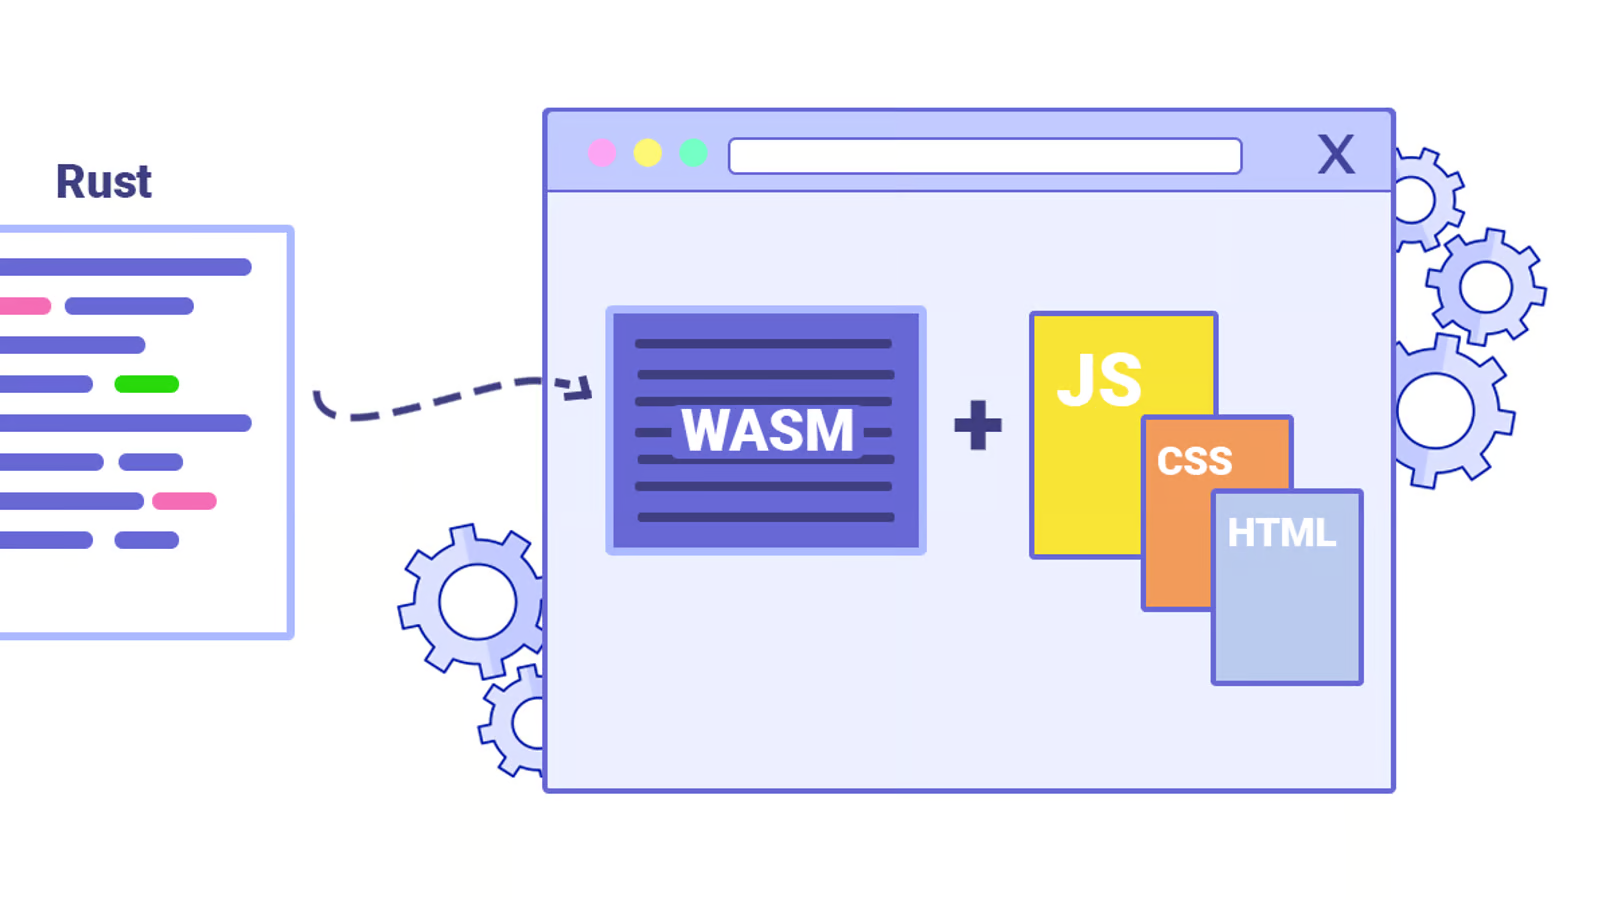
\includegraphics[width=0.7\linewidth]{./figs/herramientas/desarrollo/wasm_rust.png}
	\caption[Interacción Rust-WebAssembly]{Interacción Rust-WebAssembly \cite{garg2023}}
    \label{fig:rust_wasm}
\end{figure}

Durante la planificación inicial del proyecto, se introdujeron los conceptos básicos del Simracing al programador para asegurar una comprensión adecuada del contexto y las necesidades del proyecto. Posteriormente, se sostuvo una reunión de acercamiento con el consultor, quien, además de competir en un equipo de Simracing, posee conocimiento y experiencia en la creación de software específico para este ámbito. En esta reunión, se discutieron elementos técnicos relevantes del Simracing, incluyendo las plataformas competitivas, los diferentes tipos de análisis, en tiempo real o a posteriori, y las herramientas existentes.

Adicionalmente, se creó el repositorio inicial en GitHub (\autoref{fig:estructura_inicial_de_directorios}) y se registró el proyecto en GitHub Projects. En esta plataforma se añadieron los objetivos preliminarmente acordados y se configuraron tanto el software como las cuentas necesarias para el desarrollo del proyecto. Este enfoque sistemático aseguró una base sólida para el desarrollo del entrenador virtual, facilitando la coordinación y la gestión eficiente del proyecto desde sus etapas iniciales.

\begin{figure}[H]
    \centering
    \begin{forest}
        for tree={
            font=\ttfamily,
            grow'=0,
            child anchor=west,
            parent anchor=south,
            anchor=west,
            calign=first,
            edge path={
                \noexpand\path [draw, \forestoption{edge}]
                (!u.parent anchor) |- (.child anchor)\forestoption{edge label};
            },
            inner sep=1pt,
            l sep=10pt,
            fit=band,
            before typesetting nodes={
                if n=1
                {insert before={[,phantom]}}
                {}
            },
            where level=0{line width=1pt}{},
            before computing xy={l=20pt},
        }
        [raíz/
            [app/ , label={right:\footnotesize (Código fuente de la aplicación completa)}
                [backend/, label={right:\footnotesize (Código fuente del backend)}]
                [frontend/, label={right:\footnotesize (Código fuente del frontend)}]
                [shared/, label={right:\footnotesize (Código fuente compartido, \textit{Shared Kernel} en \ac{ddd})}]
            ]
            [docs/, label={right:\footnotesize (Documentación del proyecto)}
                [drafts/, label={right:\footnotesize (Borradores con información relevante)}]
                [report/, label={right:\footnotesize (Código fuente \LaTeX de este documento)}]
            ]
            [.gitignore, label={right:\footnotesize (Definición de los ficheros que no forman parte del proyecto)}]
            [LICENSE, label={right:\footnotesize (Definición de la licencia del proyecto)}]
            [README.md, label={right:\footnotesize (Documentación técnica sobre qué es el proyecto y cómo usarlo)}]
        ]
    \end{forest}
    \caption{Estructura inicial de directorios}
    \label{fig:estructura_inicial_de_directorios}
\end{figure}

\section{Hito 1: Adquisición y procesamiento de datos de telemetría \textit{(SO1)}}
Esta hito abarcó las actividades relacionadas con la adquisición y procesamiento de datos de telemetría, esenciales para el desarrollo del entrenador virtual de Simracing. Se investigaron los formatos de ficheros de telemetría más comunes, se desarrolló un módulo para la carga de estos ficheros y se implementaron algoritmos para la extracción e interpretación de información relevante. La validación de los datos extraídos se realizó mediante su presentación en formato tabular, asegurando la integridad y usabilidad de la información procesada. En la \autoref{tab:resumen_hito_1} se muestra un resumen del primer hito. Se debe recordar que los sprints son semanales por le que este hito abarcaría de las semanas 1 a la 9. 

\begin{table}[H]
\centering
\begin{tabular}{|l|c|}
\hline
\textbf{Título} & Adquisición y procesamiento de datos de telemetría \\ \hline
\textbf{Código} & \textit{SO1} \\ \hline
\textbf{Historias de Usuario} & 4 \\ \hline
\textbf{Sprints} & 1-9 \\ \hline
\end{tabular}
\caption{Resumen del Hito 1}
\label{tab:resumen_hito_1}
\label{tab
}
\end{table}

A continuación, se detallarán las historias de usuario desarrolladas para la adquisición y procesamiento de datos de telemetría, especificando sus objetivos, prioridades y tiempos de implementación.

\subsection{Investigación de los formatos más utilizados en ficheros de telemetría}
\begin{table}[H]
\centering
\begin{tabular}{|l|p{10cm}|}
\hline
\multicolumn{2}{|c|}{\textbf{Historia de Usuario 1}} \\ \hline
\textbf{Nombre:} & Investigar formatos comunes de ficheros de telemetría \\ \hline
\textbf{Descripción:} & Como cliente del proyecto, quiero que se identifiquen y evalúen los formatos de ficheros de telemetría más utilizados en la industria del Simracing, para seleccionar el más adecuado para este proyecto. \\ \hline
\textbf{Prioridad:} & P1 \\ \hline
\textbf{Talla:} & S \\ \hline
\textbf{Sprints:} & 1 \\ \hline
\end{tabular}
\caption{Historia de Usuario 1}
\label{tab:us_telemetria}
\end{table}

En el proceso de investigación para determinar los formatos de ficheros de telemetría más utilizados en la industria del Simracing, se realizó un análisis exhaustivo de las opciones disponibles. Se descubrió que la gran mayoría de simuladores expone sus datos de telemetría en formatos específicos, que pueden ser transformados en formatos tabulares para facilitar su análisis a posteriori.

\subsubsection*{Principales Formatos de Telemetría}
\begin{itemize}
    \item \textbf{Formato \ac{ibt}}: El formato .ibt es utilizado por iRacing para almacenar datos de telemetría. Estos ficheros contienen una gran cantidad de información detallada sobre las carreras, incluyendo datos de velocidad, revoluciones por minuto, posición en la pista, entre otros. Este formato es binario y se utiliza principalmente para análisis a posteriori, donde los datos se pueden convertir a formatos tabulares como \ac{csv} para facilitar su procesamiento y análisis.

    \item \textbf{Formato Motec}: Motec es otro formato comúnmente utilizado en simuladores como rFactor y Project CARS. Los datos de telemetría se almacenan en archivos binarios que pueden ser leídos por el software Motec, permitiendo un análisis detallado de las sesiones de carrera. Al igual que el formato \ac{ibt}, los datos pueden ser exportados a formatos tabulares para la realización de un  análisis más intuitivo.
    
    \item \textbf{Formato \ac{acti}}: Assetto Corsa utiliza el formato \ac{acti} para exponer datos de telemetría. Este formato permite la recolección de datos detallados sobre el rendimiento del vehículo y el comportamiento en pista. Los datos de \ac{acti} también pueden ser convertidos a formatos tabulares.
\end{itemize}

\subsubsection*{Análisis en Tiempo Real vs. Análisis a Posteriori}

Durante la investigación, se distinguió entre los análisis en tiempo real y los análisis a posteriori:

\begin{itemize}
    \item \textbf{Análisis en Tiempo Real}: Utiliza el \ac{sdk} proporcionado por los desarrolladores de juegos que permiten acceder a datos de telemetría en tiempo real. Estos \ac{sdk}s son esenciales para aplicaciones que requieren actualizaciones instantáneas, como paneles de control en vivo y herramientas de monitorización durante las carreras. Ejemplos incluyen el \ac{sdk} de iRacing y la \ac{api} de Telemetría de Assetto Corsa.
    \item \textbf{Análisis a Posteriori}: Este tipo de análisis se realiza una vez finalizada la sesión de simulación. Los datos de telemetría se guardan en formatos binarios como \ac{ibt} y Motec y luego se convierten a tablas para su análisis detallado. Existen diversas herramientas específicas para realizar esta conversión y facilitar el análisis.
\end{itemize}

\subsubsection*{Uso de \ac{ibt} de iRacing}
Se justificó el uso del formato \ac{ibt} de iRacing en el proyecto debido a las siguientes razones:

\begin{itemize}
    \item \textbf{Compatibilidad y Popularidad}: El formato \ac{ibt} es ampliamente utilizado en la comunidad de iRacing, garantizando una gran cantidad de recursos y herramientas disponibles para su análisis.
    \item \textbf{Detalle y Precisión}: Proporciona datos de telemetría extremadamente detallados y precisos, esenciales para realizar análisis profundos que mejoren el rendimiento del usuario en el simulador.
    \item \textbf{Integración con Herramientas Existentes}: Numerosas herramientas y librerías soportan el formato \ac{ibt}, lo que facilita su integración en el flujo de trabajo del proyecto y permite aprovechar las capacidades de análisis avanzadas que estas herramientas ofrecen.
    \item \textbf{Futuro análisis en tiempo real}: Aunque podrían haberse utilizado datos tabulares directamente, se eligió el formato \ac{ibt} para permitir futuros análisis en tiempo real. En la propuesta del proyecto, se destacó esta opción como potencialmente interesante para mejorar la flexibilidad y alcance del análisis de datos en Simracing.
\end{itemize}

\subsubsection*{Adquisición de Ficheros de Telemetría}

Para obtener los ficheros \ac{ibt} de telemetría es necesario tener una suscripción de pago a iRacing, además de contar con un equipo hardware de elevado coste para la conducción. La colaboración del consultor fue crucial en este contexto. No solo nos guió en la investigación, sino que también nos proporcionó un fichero de telemetría de un entrenamiento, permitiéndonos avanzar ágilmente en los siguientes pasos del proyecto. Su intervención subrayó la importancia de contar con un experto en la materia para optimizar procesos y asegurar la calidad del desarrollo.


\subsection{Desarrollar un módulo para la carga de ficheros de telemetría}
\begin{table}[H]
\centering
\begin{tabular}{|l|p{10cm}|}
\hline
\multicolumn{2}{|c|}{\textbf{Historia de Usuario 2}} \\ \hline
\textbf{Nombre:} & Desarrollar un módulo para la carga de ficheros de telemetría \\ \hline
\textbf{Descripción:} & Como cliente del proyecto, quiero que se desarrolle un módulo de software que permita la carga y procesamiento de ficheros de telemetría en el sistema, utilizando el formato seleccionado y asegurando la integridad y validez de los datos importados. \\ \hline
\textbf{Prioridad:} & P0 \\ \hline
\textbf{Talla:} & XL \\ \hline
\textbf{Sprints:} & 2-6 \\ \hline
\end{tabular}
\caption{Historia de Usuario 2}
\label{tab:us_carga_telemetria}
\end{table}

\subsubsection*{Investigación y selección de herramientas}
El primer paso en el desarrollo del módulo para la carga de ficheros de telemetría fue investigar las herramientas existentes que pudieran facilitar este proceso. Se identificó inicialmente la herramienta itelem \cite{itelem}, disponible en GitHub, que parecía cumplir con los requisitos del proyecto. Sin embargo, al intentar extraer la información del fichero de prueba proporcionado por el consultor, itelem mostró errores no controlados \cite{rust_panic_2023}, indicando una inadecuada gestión de errores y una falta de robustez necesaria para el manejo de datos de telemetría.

Para verificar que el problema no se debía a un fichero corrupto, se utilizó la librería JavaScript ibt-telemetry \cite{ibt-telemetry}, que logró extraer datos sin errores aparentes. No obstante, al examinar los resultados se detectaron incoherencias en el formato de fechas, además de que esta librería solo obtenía un subconjunto de todas las variables almacenadas en el fichero \ac{ibt}.

Ante las limitaciones de las herramientas anteriores, se decidió recurrir a una fuente más fiable: un clon en lenguaje C del \ac{sdk} oficial (no público) de iRacing \cite{irsdk}, disponible en GitHub. Este \ac{sdk}  es conocido por su precisión y fiabilidad en la extracción de datos de telemetría, no obstante, está diseñado para interactuar con el simulador en tiempo real. Tras un estudio detallado del mismo, se decidió utilizar esta herramienta como base para el desarrollo del módulo.

\subsubsection*{Estructura de un fichero \ac{ibt}}

Los ficheros \ac{ibt} son capturas de la memoria del simulador y se dividen en dos partes principales, que corresponden con los tipos de memoria en las que se almacena un programa: la estática y la dinámica. La memoria estática almacena datos que se conocen y determinan antes de que el programa comience a ejecutarse, mientras que la memoria dinámica se refiere a los datos que se generan y gestionan mientras el programa está en funcionamiento.

\subsubsection*{Memoria estática}

La \autoref{fig:cabecera_ibt} muestra la disposición de los diferentes componentes de la memoria estática, destacando la cabecera del fichero, los búferes de datos y la cabecera de disco, así como los elementos de alineamiento (padding) necesarios para mantener la integridad de los datos a nivel palabra de memoria.

\begin{figure}[H]
	\centering
	\includegraphics[width=1\linewidth]{./figs/herramientas/desarrollo/ibt_header.png}
	\caption[Cabeceras de un fichero IBT]{Cabeceras de un fichero \ac{ibt}}
    \label{fig:cabecera_ibt}
\end{figure}

\begin{itemize}
    \item \textbf{Cabecera}: incluye información fundamental sobre la versión, el estado, la velocidad de tick, la actualización de sesión y el tamaño y desplazamiento de diferentes segmentos de datos. Esta estructura permite al sistema gestionar y procesar la telemetría de manera eficiente, asegurando que todos los parámetros relevantes sean capturados y almacenados correctamente. Dentro de la cabecera se encuentran:
    \begin{itemize}
        \item \textbf{Información sobre el simulador}: como la versión, el estado, la velocidad de tick, la marca de actualización, etc.
        \item \textbf{Información sobre la sesión}: mediante el desplazamiento en bytes indicado se alcanza la zona donde está la información de la sesión. El campo de tamaño de información de sesión indica el número de bytes que ésta ocupa. La información de la sesión viene codificada en \ac{yaml}.
        \item \textbf{Cabeceras de las variables}: mediante el desplazamiento en bytes indicado se alcanza la zona donde están las cabeceras de las variables. Estas cabeceras tienen un tamaño fijo e indican el nombre, el tipo, la unidad y la descripción de cada variable medida. El campo de número de variables indica cuantas variables distintas son almacenadas en el fichero.
        \item \textbf{Búferes de variables}: Existen 4 búferes, cada uno con un tamaño de 16 bytes. Para extraer los datos más recientes, se selecciona el búfer con el mayor contador de ticks. Luego, se realiza un desplazamiento en el fichero según lo indicado en el búfer, encontrando así el estado más actual de las variables.
    \end{itemize}
    \item \textbf{Cabecera de disco}: Contiene información sobre la fecha de inicio, la hora de inicio y finalización en formato Unix Timestamp  de la captura de telemetría. Además, indica el número de vueltas al circuito capturadas así como el número de registros guardados.
\end{itemize}

\subsubsection*{Memoria dinámica}

Los elementos dinámicos de un fichero \ac{ibt} son:

\begin{itemize}
    \item \textbf{Información de la sesión}: La información de la sesión en los ficheros \ac{ibt} se almacena codificada en formato \ac{yaml}. Para acceder a esta información, es necesario desplazarse a la posición del fichero indicada por el valor del campo 'desplazamiento info. de sesión'. El número de bytes que se deben tomar para extraer este campo también está indicado por el campo 'desplazamiento info. de sesión'. Una vez identificada la posición y la longitud, se extrae esta sección del fichero y se decodifica como \ac{yaml}.
    
    Durante este proceso, se descubrió que la herramienta itelem presentaba un fallo al asumir que la estructura del \ac{yaml} era siempre la misma. Sin embargo, al tratarse de un campo dinámico, los campos pueden variar entre diferentes sesiones. En este proyecto, se tuvo en cuenta esta variabilidad para evitar errores similares, implementando un sistema que maneje adecuadamente estas diferencias en la estructura del \ac{yaml}.

    De manera general, este campo incluye detalles sobre la sesión de carrera, como:
    \begin{itemize}
        \item \textbf{Información del fin de semana}: Nombre y configuración del circuito, condiciones meteorológicas, y la serie o campeonato en el que se compite. Por ejemplo, podría indicar que la carrera se lleva a cabo en el ''Daytona International Speedway'' con condiciones de pista húmeda y una temperatura ambiente de 20°C.
        \item \textbf{Información de la sesión}: Detalles sobre las sesiones de práctica, clasificación y carrera, incluyendo los tiempos de inicio y fin, la duración, y el tipo de sesión. Un ejemplo sería una sesión de práctica que comienza a las 14:00 y tiene una duración de 60 minutos.
        \item \textbf{Información del conductor y del coche}: Datos sobre el piloto, el equipo y la configuración del coche. Esto puede incluir el nombre del piloto, el coche utilizado y ajustes específicos como la presión de los neumáticos y la configuración del ala trasera.
    \end{itemize}
    \item \textbf{Cabeceras de las Variables}: El desplazamiento y el número de variables se obtienen de la cabecera principal del fichero. Para acceder a las cabeceras de las variables, se lee desde el desplazamiento especificado un número de bloques igual al número de variables presentes. Cada cabecera de variable tiene un tamaño constante, definido en el código fuente.

    El tamaño de cada cabecera es constante y ocupa 144 bytes. Esto incluye diferentes campos que describen la variable, tales como el tipo de datos, el desplazamiento desde el inicio del buffer, el número de muestras que contienen esta variable, y detalles adicionales como el nombre, la descripción y la unidad de medida de la variable.

    \item \textbf{Valores de las Variables}: El proceso de extracción de los valores de las variables almacenadas en la memoria dinámica de un fichero \ac{ibt} se realiza teniendo en cuenta el desplazamiento del búfer con el contador de ticks más alto. Este contador indica que el búfer contiene los datos más recientes y, por tanto, es el punto de partida adecuado para la extracción de valores. Se comienza desde el desplazamiento indicado por el búfer seleccionado. Este desplazamiento se utiliza como punto de inicio para la lectura de los valores de las variables. Por cada cabecera de variable, se toma una cantidad de bytes igual al tipo de dato especificado en la cabecera. El tipo de dato determina el tamaño de los bytes que se deben leer para esa variable específica. Los valores se extraen consecutivamente en el orden de aparición de las cabeceras. Este proceso continúa hasta llegar al final del fichero.
\end{itemize}

\subsubsection*{Implementación}

Para desarrollar la lectura de ficheros \ac{ibt} en Rust, se ha implementado una arquitectura modular que permite una alta flexibilidad y extensibilidad del sistema. La estructura principal, File, se ha diseñado para manejar tanto la lectura de ficheros como la posibilidad de procesar datos en tiempo real, gracias a su enfoque genérico en la entrada. Este diseño permite que el sistema no esté limitado únicamente a la lectura de ficheros, sino que también pueda adaptarse para procesar flujos de datos en tiempo real.

El desarrollo se ha llevado a cabo mediante la definición de varios módulos específicos, cada uno encargado de una parte particular del fichero \ac{ibt}:

\begin{itemize}
    \item \textbf{disk\_header}: Gestiona la cabecera del disco, incluyendo la fecha y hora de inicio y fin de la grabación, el número de vueltas y el total de registros.
    \item \textbf{from\_reader}: Define las interfaces para leer tamaños fijos y variables de datos.
    \item \textbf{header}: Gestiona la cabecera principal del fichero, incluyendo la versión, el estado, la velocidad de tick, y otros parámetros cruciales.
    \item \textbf{variables} y \textbf{var\_header}: Gestionan las variables dinámicas del fichero, incluyendo la definición y los valores de las mismas.
    \item \textbf{session\_info}: Procesa la información de la sesión, que está codificada en \ac{yaml}.
    \item \textbf{var\_filter}: Aplica filtros para seleccionar solo las variables más relevantes.
\end{itemize}

La secuencia de operaciones seguida por el proceso de lectura implementado es la siguiente:

\begin{itemize}
    \item \textbf{Cabeceras}: Las cabeceras del fichero y del disco se leen primero, utilizando métodos definidos en sus respectivos módulos.
    \item \textbf{Información de la Sesión}: A continuación, se extrae la información de la sesión, desplazándose a la posición indicada y leyendo el contenido en formato \ac{yaml}.
    \item \textbf{Variables}: Finalmente, se leen las métricas desde el fichero. Se aplica un filtro predefinido para seleccionar las variables más relevantes, pero el sistema está diseñado para que esta lista de variables pueda modificarse fácilmente en el futuro.
\end{itemize}

Se han definido varios tipos de errores que pueden ocurrir durante la lectura del fichero, cada uno asociado a una parte específica del proceso, cabeceras, información de sesión, métricas, etc. Estos errores se gestionan mediante el uso de Result en Rust, asegurando un manejo robusto y descriptivo de posibles fallos.

\subsection{Desarrollar algoritmos para la extracción e interpretación de información relevante}
\begin{table}[H]
\centering
\begin{tabular}{|l|p{10cm}|}
\hline
\multicolumn{2}{|c|}{\textbf{Historia de Usuario 3}} \\ \hline
\textbf{Nombre:} & Desarrollar algoritmos para la extracción e interpretación de información relevante \\ \hline
\textbf{Descripción:} & Como cliente del proyecto, quiero que se creen algoritmos que permitan extraer e interpretar la información relevante de los datos de telemetría. \\ \hline
\textbf{Prioridad:} & P1 \\ \hline
\textbf{Talla:} & M \\ \hline
\textbf{Sprints:} & 7-8 \\ \hline
\end{tabular}
\caption{Historia de Usuario 3}
\label{tab:us_extraccion_interpretacion}
\end{table}

Para abordar esta tarea, partiendo de la información extraída en crudo del fichero \ac{ibt}, se modelaron estructuras de datos que representan los datos de telemetría de manera que pueden ser consumidos eficientemente por algoritmos de análisis, facilitando así su procesamiento y evaluación. Estas estructuras permiten una interpretación más clara y precisa de la información, facilitando su posterior análisis y utilización.

El proceso comenzó con la construcción de un modelo de datos que encapsula las variables extraídas, organizándolas de forma que reflejen la naturaleza y el contexto de los datos de telemetría. En la \autoref{fig:modelo_de_datos} se muestra un diagrama con dicho modelo.

\begin{figure}[H]
	\centering
	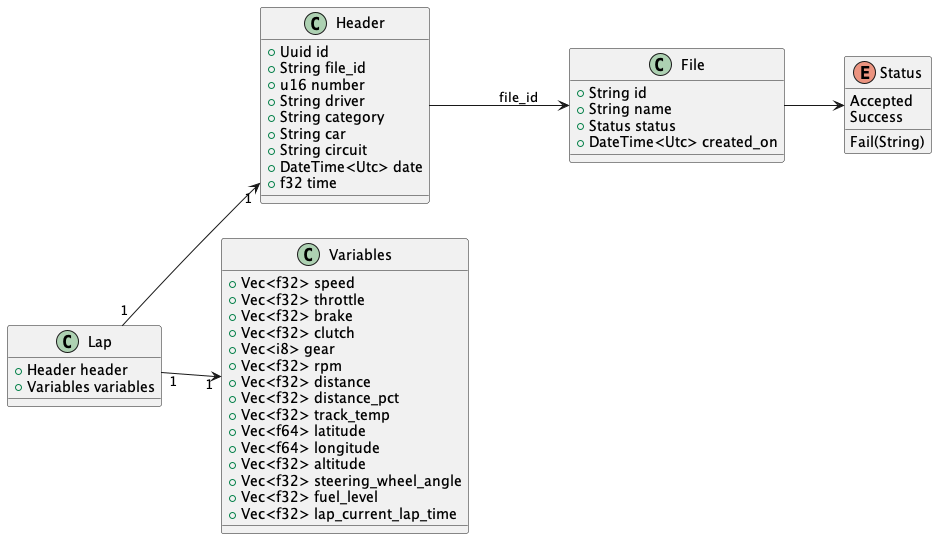
\includegraphics[width=1\linewidth]{./figs/herramientas/desarrollo/modelo_de_datos.png}
	\caption[Modelo de Datos]{Modelo de Datos}
    \label{fig:modelo_de_datos}
\end{figure}

En el diseño del modelo de datos, se tomaron decisiones clave para optimizar la eficiencia y la escalabilidad del sistema. El identificador (id) de cada File se calculó utilizando la función SHA256 sobre los bytes en bruto del fichero, garantizando así unicidad y seguridad. Además, se incluyó un estado (status) en la estructura File, permitiendo gestionar el procesamiento de archivos de manera asíncrona y facilitando la consulta del estado actual de cada archivo.

Se decidió dividir la información de una Lap en dos componentes: cabecera (Header) y datos (Variables). Esta separación permite consultar únicamente las cabeceras sin necesidad de cargar los datos completos, optimizando las consultas y mejorando el rendimiento, dado que los datos son considerablemente más pesados.

La información extraída originalmente del fichero \ac{ibt} almacena los datos en formato de filas, donde cada registro o fila contiene un valor para cada una de las variables medidas, ordenados consecutivamente según las cabeceras. Se implementó un algoritmo (\autoref{alg:from_reader}) para transformar estos datos a un formato columnar, almacenando cada variable en vectores separados. Esto permitió un acceso más eficiente a columnas específicas y optimizó las operaciones de análisis, mejorando el rendimiento del procesamiento de datos.

\IncMargin{1em}
\begin{algorithm}[H]
\SetKwInOut{Input}{Datos}
\SetKwInOut{Output}{Resultado}
\LinesNumbered
\SetAlgoLined

\Input{lector (\texttt{reader}), cabecera (\texttt{header}), filtro (\texttt{filter})}
\Output{Lista de Variables (\texttt{variables})}

\SetKwFunction{FMain}{from\_reader}
\SetKwProg{Fn}{Función}{:}{}

\Fn{\FMain{\texttt{reader}, \texttt{header}, \texttt{filter}}} {
    Leer cabeceras de variables (\texttt{var\_headers}) mediante lector y cabecera\;
    
    Calcular tamaño del bloque de variables (\texttt{var\_block\_size})\;

    \If{filtro está presente (\texttt{filter})} {
        Filtrar cabeceras de variables usando el filtro\;
    }

    \texttt{variables\_result} $\leftarrow$ lista vacía\;

    \ForEach{cabecera de variable en \texttt{var\_headers}} {
        Seleccionar el búfer con el mayor \texttt{tick\_count} de la cabecera\;
        Leer variables mediante lector, cabecera de variable, desplazamiento del búfer y tamaño del bloque de variables\;
        Añadir variable a \texttt{variables\_result}\;
    }

    \Return{Lista de Variables (\texttt{variables\_result})}\;
}
\caption{Conversión de formato \ac{ibt} a formato columnar}\label{alg:from_reader}
\end{algorithm}
\DecMargin{1em}


Las variables relativas al piloto, circuito, fecha y categoría se extrajeron de la información de la sesión utilizando la librería serde\_yaml \cite{serde_yaml}. Se implementaron estructuras de datos que permitían valores nulos, proporcionando flexibilidad para manejar el formato dinámico de almacenamiento del fichero \ac{ibt}. Esta flexibilidad fue crucial para asegurar una correcta interpretación y visualización de los datos extraídos. En el \autoref{alg:ibt_variables2laps} se muestra una parte ilustrativa del algoritmo de extracción.

\IncMargin{1em}
\begin{algorithm}[H]
\SetKwInOut{Input}{Datos}
\SetKwInOut{Output}{Resultado}
\LinesNumbered
\SetAlgoLined

\Input{Identificador de archivo (\texttt{file\_id}), información de la sesión (\texttt{session\_info}), variables extraídas (\texttt{variables})}
\Output{Lista de vueltas (\texttt{laps\_vec})}

\SetKwFunction{FMain}{ibt\_variables2laps}
\SetKwProg{Fn}{Función}{:}{}

\Fn{\FMain{\texttt{file\_id}, \texttt{session\_info}, \texttt{variables}}} {
    Obtener \texttt{driver\_name} de \texttt{session\_info}\;
    
    Obtener \texttt{category} de \texttt{session\_info}\;

    Obtener \texttt{car} de \texttt{session\_info}\;

    Obtener \texttt{circuit} de \texttt{session\_info}\;

    Obtener \texttt{date} de \texttt{session\_info}\;

    Agrupar \texttt{variables} por número de vuelta en \texttt{variables\_by\_lap}\;

    \texttt{laps\_vec} $\leftarrow$ lista vacía\;

    \ForEach{(número\_de\_vuelta, variables) en \texttt{variables\_by\_lap}} {
        Crear nueva vuelta con los parámetros \texttt{file\_id}, \texttt{número\_de\_vuelta}, \texttt{driver\_name}, \texttt{category}, \texttt{car}, \texttt{circuit}, \texttt{date} y \texttt{variables}\;
        Agregar vuelta a \texttt{laps\_vec}\;
    }

    \Return{\texttt{laps\_vec}}\;
}
\caption{Conversión de variables de IBT a vueltas}\label{alg:ibt_variables2laps}
\end{algorithm}
\DecMargin{1em}



\subsection{Validación de datos extraídos en formato tabular}
\begin{table}[H]
\centering
\begin{tabular}{|l|p{10cm}|}
\hline
\multicolumn{2}{|c|}{\textbf{Historia de Usuario 4}} \\ \hline
\textbf{Nombre:} & Validación de datos extraídos en formato tabular \\ \hline
\textbf{Descripción:} & Como cliente del proyecto, quiero visualizar los datos de telemetría extraídos en un formato tabular legible, para facilitar la validación de la información procesada y asegurar su precisión y coherencia. \\ \hline
\textbf{Prioridad:} & P2 \\ \hline
\textbf{Talla:} & S \\ \hline
\textbf{Sprints:} & 9 \\ \hline
\end{tabular}
\caption{Historia de Usuario 4}
\label{tab:us_visualizacion_basica}
\end{table}

Se determinó que, debido a la naturaleza de los datos, el formato \ac{json} es más conveniente que un formato tabular tradicional. Los datos de telemetría contienen múltiples variables con diferentes tipos y tamaños, que se capturan en intervalos muy cortos de tiempo, lo que resulta en un volumen de datos elevado y estructurado de manera compleja. Un formato tabular al uso, como  \ac{csv}, puede resultar en una representación menos clara y más difícil de manejar debido a la extensión horizontal que tendría, al intentar representar cada variable como una columna.

El formato \ac{json}, por otro lado, permite una representación jerárquica y estructurada de los datos, facilitando su organización y lectura. Al utilizar \ac{json}, cada variable de telemetría puede ser representada como una clave con sus valores correspondientes, agrupados de manera que refleje la estructura lógica de los datos. Esto no sólo mejora la legibilidad, sino que también permite una manipulación más eficiente de los datos mediante herramientas y bibliotecas de software comúnmente utilizadas en análisis de datos y desarrollo web.

Para la creación del archivo \ac{json}, se implementó un algoritmo que recorrió la estructura de datos utilizada para almacenar la telemetría extraída. Durante este proceso, los datos fueron escritos directamente en la salida estándar (stdout) en formato \ac{json}, utilizando funciones de serialización disponibles en el lenguaje de programación Rust. Esta metodología garantizó que los datos se capturaran de manera fiel y precisa, permitiendo su validación inmediata. La utilización de stdout para la generación del \ac{json} aseguró que el proceso fuera eficiente y que los datos pudieran ser redirigidos o almacenados según fuera necesario, sin necesidad de almacenamiento intermedio en archivos temporales.

En el \autoref{lst:muestra_datos_extraidos} se muestra un ejemplo del \ac{json} generado, mostrando cómo se estructuraron y visualizaron los datos de telemetría extraídos, asegurando su precisión y coherencia para facilitar su validación.

\newpage

\begin{lstlisting}[label=lst:muestra_datos_extraidos, caption=Muestra \ac{json} de los datos extraídos]
{
  "id": "123e4567-e89b-12d3-a456-426614174000",
  "file_id": 
  "e3b0c44298fc1c149afbf4c8996fb92427ae41e4649b934ca495991b7852b855",
  "number": 1,
  "driver": "John Doe",
  "category": "GT3",
  "car": "Ferrari 488 GT3",
  "circuit": "Monza",
  "date": "2024-06-19T19:15:25.258553Z",
  "time": 85.23,
  "speed": [50.2, 60.4, 70.1],
  "throttle": [0.8, 0.9, 1.0],
  "brake": [0.1, 0.0, 0.2],
  "clutch": [0.0, 0.0, 0.1],
  "gear": [3, 4, 5],
  "rpm": [7000, 7200, 7400],
  "distance": [3000.0, 3100.0, 3200.0],
  "distance_pct": [0.85, 0.88, 0.90],
  "track_temp": [28.0, 28.5, 29.0],
  "latitude": [45.467, 45.468, 45.469],
  "longitude": [9.191, 9.192, 9.193],
  "altitude": [150.0, 155.0, 160.0],
  "steering_wheel_angle": [0.05, 0.04, 0.03],
  "fuel_level": [15.0, 14.5, 14.0],
  "lap_current_lap_time": [85.23, 85.50, 85.75]
}
\end{lstlisting}

\section{Hito 2: Definición de las métricas de comparación \textit{(SO2)}}
El hito implicó un enfoque integral para establecer y comparar el rendimiento entre distintos archivos de telemetría. Inicialmente se identificaron y definieron métricas de rendimiento clave, proporcionando una base sólida para la evaluación. Posteriormente, se desarrollaron algoritmos específicos para calcular y comparar estas métricas, asegurando la precisión y coherencia en el análisis. Finalmente, se implementaron visualizaciones comparativas que permitieron una mejor comprensión y análisis de los datos, facilitando la validación y asegurando la calidad de la información procesada. 

\begin{table}[H]
\centering
\begin{tabular}{|l|c|}
\hline
\textbf{Título} & Definición de las métricas de comparación \\ \hline
\textbf{Código} & \textit{SO2} \\ \hline
\textbf{Historias de Usuario} & 3 \\ \hline
\textbf{Sprints} & 10-19 \\ \hline
\end{tabular}
\caption{Resumen del Hito 2}
\label{tab:resumen_hito_2}
\end{table}

A continuación, se detallan las historias de usuario necesarias para alcanzar el hito de la definición de las métricas de comparación. Estas historias de usuario abarcan la identificación de métricas relevantes, el desarrollo de algoritmos para su cálculo y la implementación de visualizaciones comparativas, garantizando así una evaluación precisa y comprensible del rendimiento.

\subsection{Definir métricas de rendimiento relevantes}
\begin{table}[H]
\centering
\begin{tabular}{|l|p{10cm}|}
\hline
\multicolumn{2}{|c|}{\textbf{Historia de Usuario 5}} \\ \hline
\textbf{Nombre:} & Definir métricas de rendimiento relevantes \\ \hline
\textbf{Descripción:} & Como cliente del proyecto, quiero definir métricas de rendimiento relevantes para comparar diferentes archivos de telemetría, con el fin de evaluar el rendimiento de manera precisa y consistente \\ \hline
\textbf{Prioridad:} & P1 \\ \hline
\textbf{Talla:} & S \\ \hline
\textbf{Sprints:} & 10 \\ \hline
\end{tabular}
\caption{Historia de Usuario 5}
\label{tab:metricas_rendimiento}
\end{table}

En esta historia de usuario se determinó que la métrica adecuada para comparar diferentes vueltas a un circuito sería la diferencia entre las variables de una vuelta de referencia y una vuelta objetivo. La vuelta de referencia, idealmente, corresponde a los tiempos óptimos al recorrer el circuito, mientras que la vuelta objetivo es la que se desea mejorar. Esta métrica es adecuada porque permite evaluar de manera precisa las áreas de mejora, comparando directamente el rendimiento ideal con el actual. Los beneficios incluyen una identificación clara de las diferencias de rendimiento y la focalización en aspectos específicos que necesitan optimización.

Para implementar esta métrica, se tomó como eje de referencia las distancias recorridas en lugar del tiempo. La razón principal es que el tiempo varía entre vueltas, debido a la naturaleza del desempeño del piloto y las condiciones del circuito, mientras que la distancia recorrida es una constante en todas las vueltas. Esto garantiza una comparación justa y precisa entre las vueltas de referencia y las vueltas objetivo.

Dado que la información obtenida de los archivos \ac{ibt} no contiene las distancias estandarizadas, sino que varían dependiendo de la máquina donde se ejecuta, fue necesario realizar un proceso de interpolación. Este proceso involucró calcular todos los puntos de distancia de ambas vueltas y luego interpolar los valores de las variables a estos puntos comunes. Esto permitió una comparación directa y precisa entre los datos de telemetría de las vueltas de referencia y las vueltas objetivo, asegurando que las diferencias en las métricas de rendimiento fueran coherentes y significativas. Este enfoque ha permitido una evaluación detallada y exacta del rendimiento en el simulador de carreras.

\subsection{Desarrollar algoritmos para calcular y comparar métricas}
\begin{table}[H]
\centering
\begin{tabular}{|l|p{10cm}|}
\hline
\multicolumn{2}{|c|}{\textbf{Historia de Usuario 6}} \\ \hline
\textbf{Nombre:} & Desarrollar algoritmos para calcular y comparar métricas \\ \hline
\textbf{Descripción:} & Como cliente del proyecto, quiero que se desarrollen algoritmos que permitan calcular y comparar las métricas de rendimiento entre diferentes archivos de telemetría, con el fin de obtener una evaluación detallada y precisa del rendimiento. \\ \hline
\textbf{Prioridad:} & P1 \\ \hline
\textbf{Talla:} & M \\ \hline
\textbf{Sprints:} & 11-13 \\ \hline
\end{tabular}
\caption{Historia de Usuario 6}
\label{tab:algoritmos_metricas}
\end{table}

Esta historia de usuario se focalizó en implementar algoritmos eficientes que permitieran realizar estas comparaciones de manera efectiva. El primer algoritmo (\autoref{alg:union_distancias}) se centró en la generación de una unión de puntos de distancia entre una vuelta de referencia y una vuelta objetivo. Este algoritmo ordenó y eliminó duplicados de las distancias registradas en ambas vueltas, permitiendo una comparación coherente. Esta unión de puntos es fundamental para normalizar las distancias entre diferentes vueltas, facilitando así una comparación precisa de los datos.

\IncMargin{1em}
\begin{algorithm}[H]
\SetKwInOut{Input}{Datos}
\SetKwInOut{Output}{Resultado}
\LinesNumbered
\SetAlgoLined

\Input{Dos vueltas \texttt{lap1} y \texttt{lap2} con sus distancias correspondientes}
\Output{Un vector de distancias unificadas y ordenadas}

\BlankLine
Inicializar un vector vacío \texttt{distances}\;
\ForEach{distancia en \texttt{lap1.variables.distance}}{
    Añadir la distancia a \texttt{distances}\;
}
\ForEach{distancia en \texttt{lap2.variables.distance}}{
    Añadir la distancia a \texttt{distances}\;
}
Ordenar \texttt{distances} de menor a mayor\;
Eliminar duplicados en \texttt{distances}\;

\BlankLine
\Return \texttt{distances}\;

\caption{Generación de la unión de puntos de distancia entre dos vueltas}
\label{alg:union_distancias}
\end{algorithm}
\DecMargin{1em}

El siguiente paso fue desarrollar un algoritmo (\autoref{alg:interpolacion}) para la interpolación lineal de los valores de las variables en función de las nuevas distancias unificadas. Este algoritmo permitió obtener valores interpolados de las variables tanto para la vuelta de referencia como para la vuelta objetivo, asegurando que los datos se compararan de manera precisa incluso cuando las muestras originales no coincidían en los mismos puntos de distancia.


\IncMargin{1em}
\begin{algorithm}[H]
\SetKwInOut{Input}{Datos}
\SetKwInOut{Output}{Resultado}
\LinesNumbered
\SetAlgoLined

\Input{Valores \texttt{values}, distancias \texttt{distances}, nuevas distancias \texttt{new\_distances}, indicador de discreción \texttt{is\_discrete}}
\Output{Vector de valores interpolados}

Inicializar un vector vacío \texttt{interpolated\_values}\;

\ForEach{\texttt{new\_distance} en \texttt{new\_distances}}{
    Encontrar la posición de \texttt{new\_distance} en \texttt{distances}\;
    \eIf{posición es 0}{
        \texttt{value} = \texttt{values[0]}\;
    }{
        \eIf{posición es igual al tamaño de \texttt{distances}}{
            \texttt{value} = \texttt{values[última posición]}\;
        }{
            \texttt{d0} = \texttt{distances[posición - 1]}\;
            \texttt{d1} = \texttt{distances[posición]}\;
            \texttt{v0} = \texttt{values[posición - 1]}\;
            \texttt{v1} = \texttt{values[posición]}\;

            \texttt{interpolated} = ((\texttt{new\_distance} - \texttt{d0}) / (\texttt{d1} - \texttt{d0})) * (\texttt{v1} - \texttt{v0}) + \texttt{v0}\;

            \eIf{\texttt{is\_discrete}}{
                \texttt{value} = \texttt{round(interpolated)}\;
            }{
                \texttt{value} = \texttt{interpolated}\;
            }
        }
    }
    Añadir \texttt{value} a \texttt{interpolated\_values}\;
}

\BlankLine
\Return \texttt{interpolated\_values}\;

\caption{Interpolación de valores entre la vuelta de referencia y la vuelta objetivo}
\label{alg:interpolacion}
\end{algorithm}
\DecMargin{1em}


Finalmente, se desarrolló un algoritmo para calcular las diferencias entre las variables de la vuelta de referencia y la vuelta objetivo. Este algoritmo comparó las variables interpoladas en cada punto de distancia, proporcionando un conjunto de métricas comparativas. Estas métricas permiten evaluar el rendimiento relativo entre ambas vueltas, identificando las áreas con diferencias significativas.

Todo lo anterior se ha materializado en una estructura de análisis denominada Analysis. Esta estructura encapsula la información y resultados obtenidos durante el proceso de comparación de vueltas.

La estructura Analysis incluye:
\begin{itemize}
    \item \textbf{Header}: Información básica sobre el análisis, como la descripción y metadatos asociados.
    \item \textbf{Reference y Target}: Las vueltas de referencia y objetivo que se están comparando, encapsuladas en la estructura ReferenceLap.
    \item \textbf{Union Distances}: Un vector de distancias comunes interpoladas, utilizado como eje de referencia para comparar las variables de las vueltas.
    \item \textbf{Differences}: Las métricas de diferencias calculadas entre las vueltas de referencia y objetivo, representadas en la estructura Variables.
\end{itemize}


Esta organización ha permitido almacenar y analizar de manera coherente los resultados comparativos, facilitando su interpretación y utilización para mejorar el rendimiento en las estrategias de conducción y configuración del vehículo. En la  \autoref{fig:modelo_de_datos_analisis} se presenta el diagrama de clases que ilustra la estructura y relaciones de la clase Analysis.

\begin{figure}[H]
	\centering
	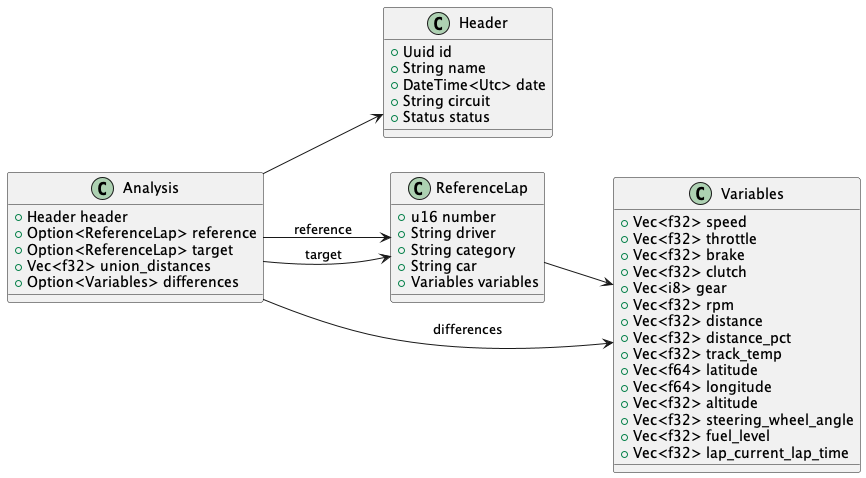
\includegraphics[width=1\linewidth]{./figs/herramientas/desarrollo/modelo_de_datos_analisis.png}
	\caption[Modelo de Datos Datos: Análisis]{Modelo de Datos: Análisis}
    \label{fig:modelo_de_datos_analisis}
\end{figure}

\subsection{Implementar visualizaciones comparativas de métricas}
\begin{table}[H]
\centering
\begin{tabular}{|l|p{10cm}|}
\hline
\multicolumn{2}{|c|}{\textbf{Historia de Usuario 7}} \\ \hline
\textbf{Nombre:} & Implementar visualizaciones comparativas de métricas \\ \hline
\textbf{Descripción:} & Como cliente del proyecto, quiero que se implementen visualizaciones comparativas de las métricas de rendimiento, para facilitar la comprensión y análisis de los datos de telemetría de manera visual y accesible. \\ \hline
\textbf{Prioridad:} & P1 \\ \hline
\textbf{Talla:} & L \\ \hline
\textbf{Sprints:} & 14-19 \\ \hline
\end{tabular}
\caption{Historia de Usuario 7}
\label{tab:metricas_rendimiento}
\end{table}

Para esta historia de usuario, se desarrollaron diversas estrategias para lograr una representación visual accesible y comprensible de los datos de telemetría. Se utilizó plotly.rs \cite{plotly}, una adaptación en Rust de la conocida librería de visualización Plotly en JavaScript \cite{plotly_js}. Inicialmente, se implementaron diagramas de dispersión utilizando la distancia como eje X y las diferentes variables de telemetría en el eje Y. Este enfoque permitió un primer módulo parcialmente funcional y estilizado para visualizar los datos.

Durante la revisión del sprint, el cliente solicitó mejoras significativas: se requería la visualización de las métricas más importantes en gráficos superpuestos, con un indicador sincronizado en todos ellos. Además, se especificó que el zoom debía ser horizontal y sincronizado entre todos los gráficos. Sin embargo, se encontraron varios desafíos técnicos con plotly.rs, ya que no permitía este comportamiento de forma nativa. Se intentó una solución manual, pero plotly.rs sólo permite gestionar eventos mediante \ac{wasm}. Al utilizar \ac{wasm}, se descubrió que los eventos emitidos por plotly no eran reconocidos. Para solucionar este problema, se habría necesitado desarrollar un proyecto completo en \ac{wasm} para gestionar estos eventos.

Para superar estos obstáculos, se decidió implementar la parte de sincronización de zoom e indicadores en JavaScript, estableciendo un enlace con Rust mediante \ac{wasm} para que ambos lenguajes pudieran comunicarse eficientemente. Este enfoque permitió implementar la funcionalidad deseada de manera efectiva.

El \autoref{lst:plotly_js} muestra el código JavaScript que implementa la sincronización del indicador de las gráficas de dispersión de Plotly cuando el puntero del ratón se posiciona sobre ellas.


\begin{lstlisting}[label=lst:plotly_js, caption=Sincronización del indicador cuando el cursor pase por encima]
export function sync_plotly(div_id, sync_div_ids) {
    let dashboardPlot = document.getElementById(div_id);
    let plotsNames = [...Object.keys(dashboardPlot._fullLayout._plots)];
    dashboardPlot.on('plotly_hover', function (event) {
        sync_div_ids.forEach(sync_div_id => {
            let syncPlot = document.getElementById(sync_div_id);
            Plotly.Fx.hover(
                syncPlot,
                { xval: event.xvals[0] },
                plotsNames
            );
            window.wasmBindings.hover_event_from_plotly(
                    event.xvals[0]
                );
        });
    });
}
\end{lstlisting}
\vspace{1em}
El \autoref{lst:wasm_bind} muestra el enlace del código anterior con código Rust mediante \ac{wasm}.

\begin{lstlisting}[language=Rust, label=lst:wasm_bind, caption=Enlace del código JavaScript a Rust mediante \ac{wasm}]
#[wasm_bindgen(module = "/assets/scripts/plotly_interop.js")]
extern "C" {
    #[wasm_bindgen(js_name = "sync_plotly")]
    fn sync_plotly(div_id: JsValue, sync_div_ids: Vec<JsValue>);
}
\end{lstlisting}

Además, se añadió un eje Y adicional a cada diagrama de dispersión para mostrar el vector de diferencias entre ambas vueltas en su escala correspondiente para cada punto de la distancia. En la \autoref{fig:visualizacion} se muestran de forma clara y detallada los puntos con mayor diferencia entre las vueltas.

\begin{figure}[H]
	\centering
	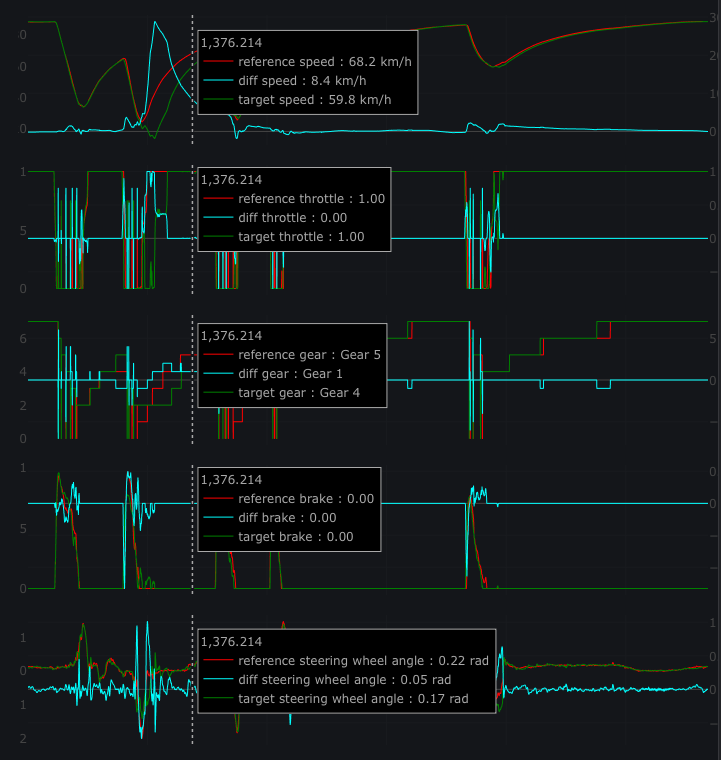
\includegraphics[width=1\linewidth]{./figs/herramientas/desarrollo/visualizacion.png}
	\caption[Visualización de diferencias de variables]{Visualización de diferencias de variables}
    \label{fig:visualizacion}
\end{figure}
\vspace{2em}

\newpage



\section{Hito 3: Aplicación de aprendizaje no supervisado \textit{(SO3)}}

En este hito se implementaron técnicas de aprendizaje no supervisado para clasificar las diferencias de las variables obtenidas de los archivos de telemetría. El objetivo fue identificar patrones y agrupar las diferencias en categorías significativas, permitiendo una evaluación detallada y precisa del rendimiento. Esta clasificación facilitó la interpretación de los datos y mejoró la comprensión de las variaciones en el rendimiento.

\begin{table}[H]
\centering
\begin{tabular}{|l|c|}
\hline
\textbf{Título} & Aplicación de aprendizaje no supervisado \\ \hline
\textbf{Código} & \textit{SO3} \\ \hline
\textbf{Historias de Usuario} & 3 \\ \hline
\textbf{Sprints} & 20-26 \\ \hline
\end{tabular}
\caption{Resumen de la sección: Aplicación de aprendizaje no supervisado}
\label{tab
}
\end{table}

A lo largo de este hito, se identificaron y evaluaron varios algoritmos de agrupamiento para seleccionar el más adecuado para clasificar las diferencias de variables. Se desarrollaron e implementaron algoritmos específicos para agrupar estas diferencias en categorías ordenadas y se abordaron problemas inherentes a los métodos seleccionados. Finalmente, se aplicaron técnicas avanzadas para mejorar la precisión y utilidad de las categorías generadas, asegurando una clasificación más precisa y adaptable de los datos de telemetría. A continuación, se detallan las historias de usuario que conformaron el hito.

\subsection{Identificación de algoritmos de agrupamiento apropiados}
\begin{table}[H]
\centering
\begin{tabular}{|l|p{10cm}|}
\hline
\multicolumn{2}{|c|}{\textbf{Historia de Usuario 8}} \\ \hline
\textbf{Nombre:} & Identificación de algoritmos de agrupamiento apropiados \\ \hline
\textbf{Descripción:} & Como cliente del proyecto, quiero identificar los algoritmos de agrupamiento más adecuados para clasificar las métricas de diferencias de las variables de telemetría, con el fin de obtener agrupamientos precisos y útiles para el análisis de rendimiento. \\ \hline
\textbf{Prioridad:} & P1 \\ \hline
\textbf{Talla:} & M \\ \hline
\textbf{Sprints:} & 20-21 \\ \hline
\end{tabular}
\caption{Historia de Usuario 8}
\label{tab:identificar_algoritmos_agrupamiento}
\end{table}

Para clasificar los vectores de diferencias en las variables de telemetría, se evaluó inicialmente el uso del algoritmo K-means debido a su simplicidad, eficiencia y capacidad para crear categorías ordenadas. K-means agrupa datos en un número predefinido de agrupaciones, donde cada punto de datos pertenece al grupo cuyo centroide es el más cercano. Este algoritmo minimiza la variabilidad dentro de cada agrupación, asegurando que los puntos de datos dentro de un grupo sean lo más similares posible. El \autoref{alg:k-means} muestra el algoritmo K-means.

\IncMargin{1em}
\begin{algorithm}[H]
\SetKwInOut{Input}{Datos}\SetKwInOut{Output}{Resultado}
\LinesNumbered
\SetAlgoLined

\Input{Conjunto de datos $\mathbf{X}$, número de clusters $k$}
\Output{Conjunto de centroides $\mathbf{C}$, asignaciones de clusters $\mathbf{A}$}

Inicializar aleatoriamente los centroides $\mathbf{C}$;
\Repeat{convergencia}{
\ForEach{punto de datos $\mathbf{x}_i$}{
Asignar el punto de datos al cluster más cercano $a_i = \arg\min_j |\mathbf{x}_i - \mathbf{c}_j|$;
}
\ForEach{cluster $j$}{
Actualizar el centroide $\mathbf{c}j = \frac{1}{|C_j|} \sum{\mathbf{x}_i \in C_j} \mathbf{x}_i$;
}
}
\caption{Algoritmo K-means}\label{alg
}
\label{alg:k-means}
\end{algorithm}
\DecMargin{1em}

La característica de K-means de ordenar las categorías es especialmente útil para clasificar diferencias en las variables de telemetría. Por ejemplo, si se determina que el número óptimo de clusters es cinco (k=5), las categorías podrían ser: ``Mucha Diferencia Negativa'', ``Diferencia Negativa'', '``No diferencia'', ``Diferencia Positiva'' y ``Mucha Diferencia Positiva''. En este caso, el primer grupo tendría centroides más cercanos a las diferencias negativas con menor valor, y así sucesivamente, asegurando que las categorías estén ordenadas de manera coherente.

\subsubsection*{Problemas identificados con K-means}
Sin embargo, K-means presenta ciertas limitaciones al crear clases cerradas. En particular, cuando los puntos de datos están cerca de los límites de dos clases, el algoritmo fuerza a que pertenezcan exclusivamente a una de ellas. Por ejemplo, si consideramos la variable velocidad y un punto de la diferencia de velocidad que está casi equidistante a los centroides de las clases ``No Diferencia'' y ``Diferencia Negativa", K-means asignaría el punto a una de las dos clases, perdiendo la información sobre su cercanía a ambas. La \autoref{fig:problemas_kmeans} refleja este problema.

\begin{figure}[H]
\centering
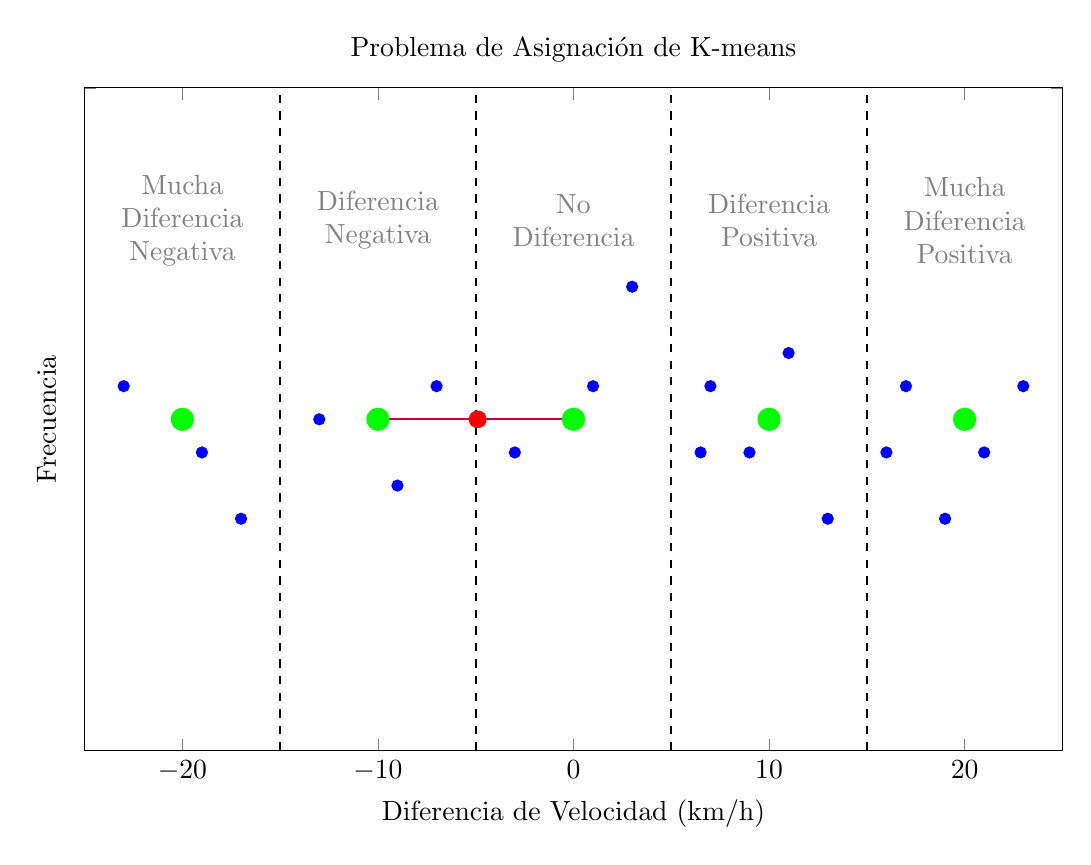
\begin{tikzpicture}
\begin{axis}[
    title={Problema de Asignación de K-means},
    xlabel={Diferencia de Velocidad (km/h)},
    ylabel={Frecuencia},
    ytick={\empty},
    xtick={-20, -10, 0, 10, 20},
    ymajorgrids=true,
    grid style=dashed,
    xmin=-25, xmax=25,
    ymin=0, ymax=1,
    enlargelimits=false,
    clip=false,
    width=14cm,
    height=10cm,
    extra y ticks={1},
    extra y tick labels={},
    extra y tick style={grid=none}
]

% Dibujar puntos de clusters
\addplot[
    only marks,
    mark=*,
    color=blue
    ]
    coordinates {
    (-23, 0.55)
    (-19, 0.45)
    (-17, 0.35)
    (-13, 0.5)
    (-9, 0.4)
    (-7, 0.55)
    (-3, 0.45)
    (1, 0.55)
    (3, 0.7)
    (6.5, 0.45)
    (7, 0.55)
    (9, 0.45)
    (11, 0.6)
    (13, 0.35)
    (16, 0.45)
    (17, 0.55)
    (19, 0.35)
    (21, 0.45)
    (23, 0.55)
    };

% Añadir el punto en cuestión
\addplot[
    only marks,
    mark=*,
    mark options={scale=1.5, fill=red},
    color=red
    ]
    coordinates {
    (-4.9, 0.5)
    };

% Añadir centroides
\addplot[
    only marks,
    mark=*,
    mark options={scale=2, fill=green},
    color=green
    ]
    coordinates {
    (-20, 0.5)
    (-10, 0.5)
    (0, 0.5)
    (10, 0.5)
    (20, 0.5)
    };

% Líneas de delimitación de clusters
\draw[dashed, thick] (axis cs:-15,0) -- (axis cs:-15,1);
\draw[dashed, thick] (axis cs:-5,0) -- (axis cs:-5,1);
\draw[dashed, thick] (axis cs:5,0) -- (axis cs:5,1);
\draw[dashed, thick] (axis cs:15,0) -- (axis cs:15,1);

% Flechas de doble punta
\draw[<->, thick, color=purple] (axis cs:-4.9,0.5) -- (axis cs:-10,0.5);
\draw[<->, thick, color=purple] (axis cs:-4.9,0.5) -- (axis cs:0,0.5);

% Etiquetas de las categorías dentro de la gráfica
\node[align=center, text=gray] at (axis cs:-20,0.8) {Mucha\\Diferencia\\Negativa};
\node[align=center, text=gray] at (axis cs:-10,0.8) {Diferencia\\Negativa};
\node[align=center, text=gray] at (axis cs:0,0.8) {No\\Diferencia};
\node[align=center, text=gray] at (axis cs:10,0.8) {Diferencia\\Positiva};
\node[align=center, text=gray] at (axis cs:20,0.8) {Mucha\\Diferencia\\Positiva};

\end{axis}
\end{tikzpicture}
\caption{Ejemplo de un punto cercano al límite entre las categorías de K-means}
\label{fig:problemas_kmeans}
\end{figure}

\subsubsection*{Resolviendo el problema mediante conjuntos difusos}
Para resolver este problema, se planteó el uso de conjuntos difusos, donde cada punto de datos puede pertenecer a múltiples clases con diferentes niveles de pertenencia. Esto permite una representación más precisa de los puntos que están en los límites de las clases. En la \autoref{fig:conjuntos_difusos} se puede ver como utilizando conjuntos difusos se captura la pertenencia a dos conjuntos, evitando la polarización de K-means.

\begin{figure}[H]
    \centering
    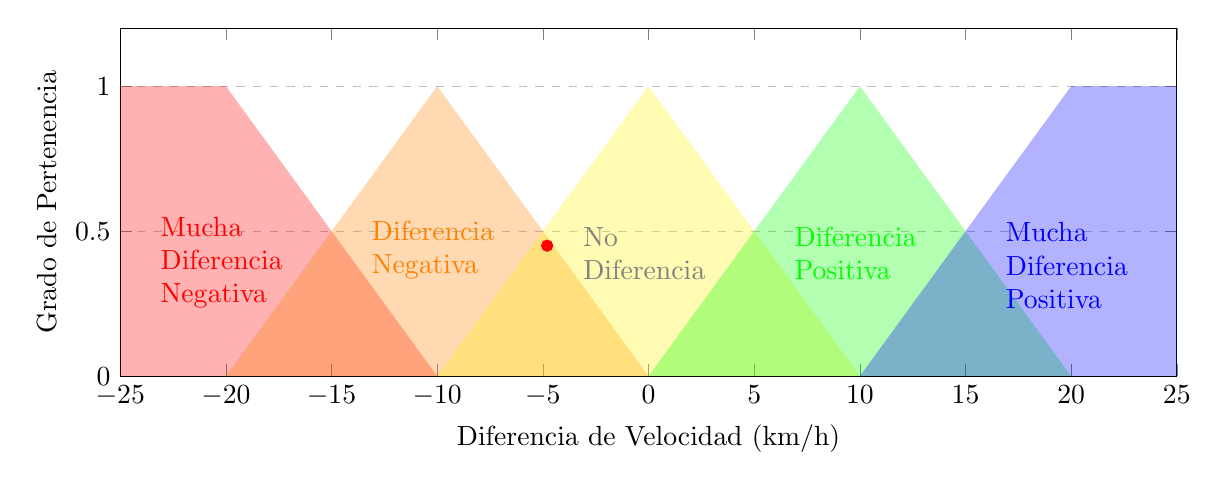
\begin{tikzpicture}
        \begin{axis}[
            width=15cm,
            height=6cm,
            xlabel={Diferencia de Velocidad (km/h)},
            ylabel={Grado de Pertenencia},
            xmin=-25, xmax=25,
            ymin=0, ymax=1.2,
            xtick={-25,-20,-15,-10,-5,0,5,10,15,20,25},
            ytick={0,0.5,1},
            ymajorgrids=true,
            grid style=dashed,
            no markers,
        ]

        % Conjuntos difusos con colores y opacidad
        \addplot[fill=red, fill opacity=0.3, draw=none] coordinates {(-25,1) (-20,1) (-10,0)} \closedcycle;
        \addplot[fill=orange, fill opacity=0.3, draw=none] coordinates {(-20,0) (-10,1) (0,0)} \closedcycle;
        \addplot[fill=yellow, fill opacity=0.3, draw=none] coordinates {(-10,0) (0,1) (10,0)} \closedcycle;
        \addplot[fill=green, fill opacity=0.3, draw=none] coordinates {(0,0) (10,1) (20,0)} \closedcycle;
        \addplot[fill=blue, fill opacity=0.3, draw=none] coordinates {(10,0) (20,1) (25,1)} \closedcycle;

        % Punto de pertenencia difusa
        \addplot[only marks, mark=*, red] coordinates {(-4.8,0.45)};

        % Etiquetas de las categorías
        \node[anchor=south, align=center] at (axis cs:-17.5,0.2) {\textcolor{red}{\parbox{3cm}{Mucha \\ Diferencia \\ Negativa}}};
        \node[anchor=south, align=center] at (axis cs:-7.5,0.3) {\textcolor{orange}{\parbox{3cm}{Diferencia \\ Negativa}}};
        \node[anchor=south, align=center] at (axis cs:2.5,0.3) {\textcolor{gray}{\parbox{3cm}{No \\ Diferencia}}}; % Etiqueta en tono más oscuro
        \node[anchor=south, align=center] at (axis cs:12.5,0.3) {\textcolor{green}{\parbox{3cm}{Diferencia \\ Positiva}}};
        \node[anchor=south, align=center] at (axis cs:22.5,0.2) {\textcolor{blue}{\parbox{3cm}{Mucha \\ Diferencia \\ Positiva}}};
        
        \end{axis}
    \end{tikzpicture}
    \caption{Conjuntos difusos aplicados a la diferencia de velocidad, con un punto ilustrativo.}
    \label{fig:conjuntos_difusos}
\end{figure}

Se consideró la posibilidad de realizar una clasificación difusa a partir de las agrupaciones generadas por K-means, lo que implicaba calcular el grado de pertenencia de cada punto a múltiples categorías. Este enfoque requería un procesamiento adicional para calcular las pertenencias difusas después de la clasificación inicial, lo que incrementaba significativamente el coste computacional y la complejidad de implementación.

En lugar de ello, se optó por utilizar directamente el algoritmo \ac{fcm}, que integra la clasificación difusa desde el principio. \ac{fcm} asigna a cada punto un grado de pertenencia a todas las categorías, reflejando de manera más precisa la incertidumbre inherente en los datos cercanos a los límites de las categorías. Esto no sólo redujo el coste computacional al eliminar la necesidad de un post-procesamiento adicional, sino que también simplificó la implementación y mejoró el rendimiento general del sistema al evitar duplicidades en el cálculo de pertenencias difusas. El \autoref{alg:fcm} muestra el funcionamiento de \ac{fcm}.

\IncMargin{1em}
\begin{algorithm}
\SetKwInOut{Input}{Datos}\SetKwInOut{Output}{Resultado}
\LinesNumbered
\SetAlgoLined

\Input{Conjunto de datos $\mathbf{X}$, número de clusters $C$, parámetro de difusidad $m$}
\Output{Matriz de pertenencia $\mathbf{U}$, centroides $\mathbf{V}$}

Inicializar aleatoriamente la matriz de pertenencia $\mathbf{U}$;
\Repeat{convergencia}{
Calcular los centroides $\mathbf{V}j = \frac{\sum{i=1}^{n} u_{ij}^m \mathbf{x}_i}{\sum{i=1}^{n} u_{ij}^m}$;\\
\ForEach{punto de datos $\mathbf{x}_i$}{
\ForEach{cluster $j$}{
Actualizar la pertenencia $u_{ij} = \frac{1}{\sum_{k=1}^{C} \left( \frac{||\mathbf{x}_i - \mathbf{v}_j||}{||\mathbf{x}_i - \mathbf{v}_k||} \right)^{\frac{2}{m-1}}}$;
}
}
}
\caption{Algoritmo Fuzzy C-means}\label{alg
}
\label{alg:fcm}
\end{algorithm}
\DecMargin{1em}

Por ejemplo, considerando nuevamente la variable velocidad, si un punto de diferencia de velocidad pertenece parcialmente a las clases ``No Diferencia'' y ``Diferencia Negativa'', \ac{fcm} asignaría niveles de pertenencia como 0.45 y 0.55 respectivamente. Esto refleja más adecuadamente la realidad del punto de datos y permite un análisis más detallado y preciso. La \autoref{fig:soluciones_fcm} muestra gráficamente la solución al problema planteado en la \autoref{fig:problemas_kmeans}. 

\begin{figure}[H]
\centering
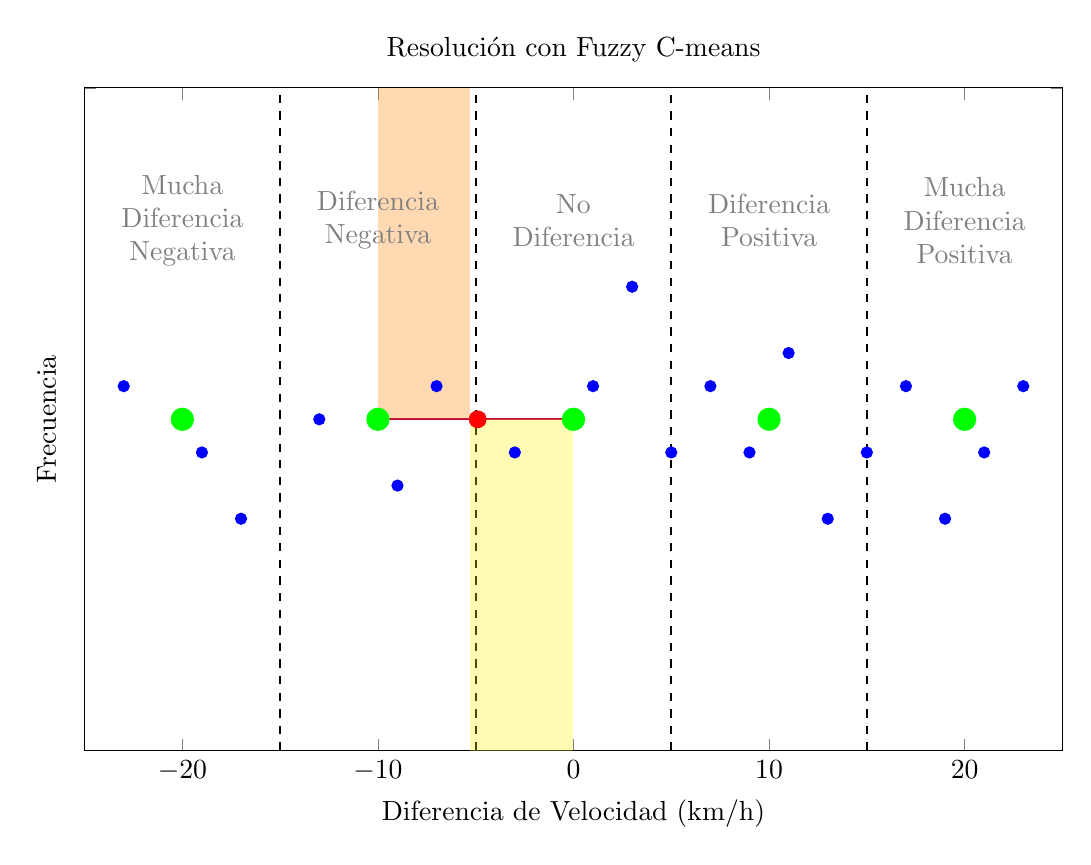
\begin{tikzpicture}
\begin{axis}[
    title={Resolución con Fuzzy C-means},
    xlabel={Diferencia de Velocidad (km/h)},
    ylabel={Frecuencia},
    ytick={\empty},
    xtick={-20, -10, 0, 10, 20},
    ymajorgrids=true,
    grid style=dashed,
    xmin=-25, xmax=25,
    ymin=0, ymax=1,
    enlargelimits=false,
    clip=false,
    width=14cm,
    height=10cm,
    extra y ticks={1},
    extra y tick labels={},
    extra y tick style={grid=none}
]

% Dibujar puntos de clusters
\addplot[
    only marks,
    mark=*,
    color=blue
    ]
    coordinates {
    (-23, 0.55)
    (-19, 0.45)
    (-17, 0.35)
    (-13, 0.5)
    (-9, 0.4)
    (-7, 0.55)
    (-3, 0.45)
    (1, 0.55)
    (3, 0.7)
    (5, 0.45)
    (7, 0.55)
    (9, 0.45)
    (11, 0.6)
    (13, 0.35)
    (15, 0.45)
    (17, 0.55)
    (19, 0.35)
    (21, 0.45)
    (23, 0.55)
    };

% Añadir el punto en cuestión
\addplot[
    only marks,
    mark=*,
    mark options={scale=1.5, fill=red},
    color=red
    ]
    coordinates {
    (-4.9, 0.5)
    };

% Añadir centroides
\addplot[
    only marks,
    mark=*,
    mark options={scale=2, fill=green},
    color=green
    ]
    coordinates {
    (-20, 0.5)
    (-10, 0.5)
    (0, 0.5)
    (10, 0.5)
    (20, 0.5)
    };

% Líneas de delimitación de clusters
\draw[dashed, thick] (axis cs:-15,0) -- (axis cs:-15,1);
\draw[dashed, thick] (axis cs:-5,0) -- (axis cs:-5,1);
\draw[dashed, thick] (axis cs:5,0) -- (axis cs:5,1);
\draw[dashed, thick] (axis cs:15,0) -- (axis cs:15,1);

% Flechas de doble punta
\draw[<->, thick, color=purple] (axis cs:-4.9,0.5) -- (axis cs:-10,0.5);
\draw[<->, thick, color=purple] (axis cs:-4.9,0.5) -- (axis cs:0,0.5);

% Representación de pertenencia difusa
\fill[opacity=0.3, color=yellow] (axis cs:-5.3, 0) rectangle (axis cs:0, 0.5);
\fill[opacity=0.3, color=orange] (axis cs:-5.3, 0.5) rectangle (axis cs:-10, 1);

% Etiquetas de las categorías dentro de la gráfica
\node[align=center, text=gray] at (axis cs:-20,0.8) {Mucha\\Diferencia\\Negativa};
\node[align=center, text=gray] at (axis cs:-10,0.8) {Diferencia\\Negativa};
\node[align=center, text=gray] at (axis cs:0,0.8) {No\\Diferencia};
\node[align=center, text=gray] at (axis cs:10,0.8) {Diferencia\\Positiva};
\node[align=center, text=gray] at (axis cs:20,0.8) {Mucha\\Diferencia\\Positiva};

\end{axis}
\end{tikzpicture}
\caption{Resolución de la asignación con conjuntos difusos usando Fuzzy C-means}
\label{fig:soluciones_fcm}
\end{figure}

\subsection{Configuración de parámetros del algoritmo de agrupamiento}
\begin{table}[H]
\centering
\begin{tabular}{|l|p{10cm}|}
\hline
\multicolumn{2}{|c|}{\textbf{Historia de Usuario 9}} \\ \hline
\textbf{Nombre:} & Configuración de parámetros del algoritmo de agrupamiento \\ \hline
\textbf{Descripción:} & Como cliente del proyecto, quiero configurar los parámetros del algoritmo de agrupamiento seleccionado para optimizar la clasificación de las diferencias en las métricas de telemetría, con el fin de obtener resultados precisos y útiles para el análisis de rendimiento. \\ \hline
\textbf{Prioridad:} & P2 \\ \hline
\textbf{Talla:} & M \\ \hline
\textbf{Sprints:} & 22-23 \\ \hline
\end{tabular}
\caption{Historia de Usuario 9}
\label{tab:configurar_algoritmos_agrupamiento}
\end{table}


En esta historia de usuario se abordó la optimización de los parámetros del algoritmo \ac{fcm} para clasificar eficazmente las diferencias en las métricas de telemetría. El objetivo fue obtener una clasificación precisa y útil para el análisis de rendimiento.

Inicialmente, el cliente propuso permitir que los usuarios configuraran los parámetros del algoritmo de agrupamiento. Sin embargo, se determinó que esta opción requería un control exhaustivo de las entradas del usuario para evitar configuraciones inadecuadas que podrían comprometer la precisión del análisis. Por esta razón, se decidió postergar esta funcionalidad para futuras implementaciones.

En su lugar, se optó por automatizar la configuración de los parámetros utilizando el \ac{fpc} como criterio de optimización. El \ac{fpc} es una medida utilizada en el análisis de conglomerados difusos para evaluar la calidad de las particiones generadas por el algoritmo \ac{fcm}. Este coeficiente varía entre 0 y 1, donde valores más altos indican una mejor definición de los conglomerados, es decir, una menor superposición entre ellos. Un \ac{fpc} cercano a 1 sería ideal, indicando particiones de alta calidad con mínima superposición entre los grupos. La \autoref{fig:fpc} muestra un ejemplo de distintos valores de \ac{fpc} en función de sus parámetros.

\begin{figure}[H]
    \centering
    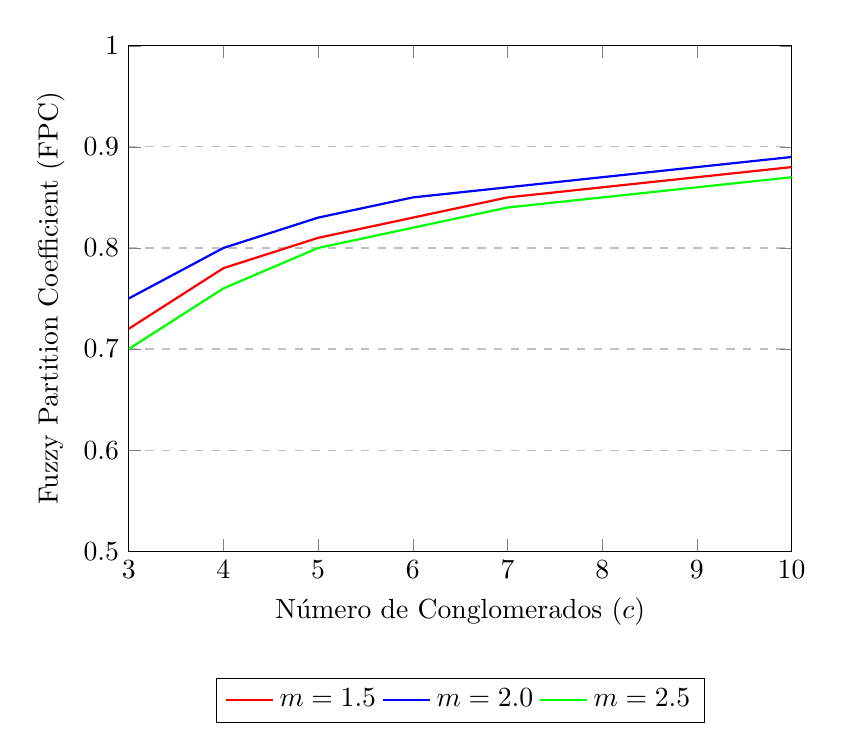
\begin{tikzpicture}
        \begin{axis}[
            width=10cm,
            height=8cm,
            xlabel={Número de Conglomerados ($c$)},
            ylabel={Fuzzy Partition Coefficient (FPC)},
            xmin=3, xmax=10,
            ymin=0.5, ymax=1,
            xtick={3,4,5,6,7,8,9,10},
            ytick={0.5,0.6,0.7,0.8,0.9,1},
            ymajorgrids=true,
            grid style=dashed,
            legend style={at={(0.5,-0.25)}, anchor=north, legend columns=-1},
            no markers,
        ]
        % FPC para m = 1.5
        \addplot[
            color=red,
            thick,
        ] coordinates {
            (3,0.72) (4,0.78) (5,0.81) (6,0.83) (7,0.85) (8,0.86) (9,0.87) (10,0.88)
        };
        % FPC para m = 2.0
        \addplot[
            color=blue,
            thick,
        ] coordinates {
            (3,0.75) (4,0.80) (5,0.83) (6,0.85) (7,0.86) (8,0.87) (9,0.88) (10,0.89)
        };
        % FPC para m = 2.5
        \addplot[
            color=green,
            thick,
        ] coordinates {
            (3,0.70) (4,0.76) (5,0.80) (6,0.82) (7,0.84) (8,0.85) (9,0.86) (10,0.87)
        };
        
        \legend{$m=1.5$,$m=2.0$,$m=2.5$}
        \end{axis}
    \end{tikzpicture}
    \caption{Fuzzy Partition Coefficient (FPC) en función del número de conglomerados ($c$) para diferentes valores de $m$.}
    \label{fig:fpc}
\end{figure}

El algoritmo \ac{fcm} tiene varios parámetros que influyen en su desempeño:

\begin{itemize}
    \item \textbf{Número de conglomerados ($c$)}: Este parámetro determina el número de categorías que se utilizarán para clasificar los datos. Es crucial seleccionar un número apropiado de conglomerados para capturar adecuadamente la estructura subyacente de los datos. En esta implementación, se evaluó típicamente entre 3 y 10, ya que tener sólo dos conglomerados no suele ser conveniente. Con solo dos conglomerados, la capacidad del algoritmo para capturar la diversidad y las variaciones en los datos es limitada, lo que puede llevar a una interpretación demasiado simplificada y posiblemente incorrecta de los datos.
    \item \textbf{Exponente de difusividad ($m$)}: Este parámetro controla el grado de difusividad de la pertenencia de los puntos a los conglomerados. Valores más altos de $m$ resultan en conglomerados más difusos. El valor de $m$ se evaluó en un rango de 1.3 a 2.5. Este rango se seleccionó por las siguientes razones:
    \begin{itemize}
        \item \textit{Claridad en la difusividad}: Valores de $m$ mayores a 2.5 tienden a producir conglomerados excesivamente difusos, disminuyendo la capacidad del algoritmo para identificar claramente las diferencias entre los grupos.
        \item \textit{Estabilidad de la clasificación}: Valores más altos pueden hacer que la clasificación sea más sensible a pequeñas variaciones en los datos, resultando en una menor estabilidad en la asignación de pertenencias.
        \item \textit{Rendimiento computacional}: Valores de $m$ más altos incrementan la complejidad computacional del algoritmo FCM. Al limitar el rango de 1,3 a 2.5, se logra un mejor rendimiento computacional sin sacrificar la calidad de los resultados.
    \end{itemize}
    \item \textbf{Criterio de convergencia}: Este parámetro, también conocido como parámetro de error, define cuándo debe detenerse el algoritmo. Normalmente, se utiliza un umbral pequeño ($\epsilon$), y el algoritmo se detiene cuando la mejora en la función objetivo entre iteraciones sucesivas es menor que este umbral. En esta implementación, se utilizó un rango de valores para $\epsilon$ entre $10^{-4}$ y $10^{-6}$ para asegurar una convergencia precisa.
    \item \textbf{Número máximo de iteraciones}: Este parámetro limita el número de iteraciones del algoritmo para prevenir ciclos infinitos. Se seleccionó un rango de valores entre 500 y 1000 iteraciones, asegurando suficiente tiempo para la convergencia sin extender innecesariamente el tiempo de cálculo.
\end{itemize}

El coeficiente de partición difusa (\ac{fpc}) se calcula utilizando la siguiente fórmula:
\[
\text{FPC} = \frac{1}{n} \sum_{i=1}^{n} \sum_{j=1}^{c} u_{ij}^2
\]
donde:
\begin{itemize}
    \item \( n \) es el número de puntos de datos,
    \item \( c \) es el número de clusters,
    \item \( u_{ij} \) es el grado de pertenencia del punto de datos \( i \) al cluster \( j \).
\end{itemize}


Para seleccionar automáticamente los valores óptimos de estos parámetros, se realizó una búsqueda en un rango apropiado. El valor óptimo de $c$ y $m$ fue el que maximizó el FPC, asegurando así la mejor calidad de las particiones difusas generadas por el algoritmo.

Mediante esta configuración automática, se garantizó que los parámetros del algoritmo FCM estuvieran optimizados para producir clasificaciones precisas y útiles, sin necesidad de intervención manual por parte del usuario. Este enfoque no sólo mejoró la precisión del análisis de telemetría, sino que también simplificó el proceso para los usuarios, asegurando resultados consistentes y de alta calidad.

\subsection{Implementación del algoritmo de Agrupamiento}
\begin{table}[H]
\centering
\begin{tabular}{|l|p{10cm}|}
\hline
\multicolumn{2}{|c|}{\textbf{Historia de Usuario 10}} \\ \hline
\textbf{Nombre:} &  Implementación del algoritmo de Agrupamiento \\ \hline
\textbf{Descripción:} & Como cliente del proyecto, quiero implementar el algoritmo de agrupamiento seleccionado para clasificar las diferencias en las métricas de telemetría, con el fin de obtener una representación precisa de los patrones de rendimiento.  \\ \hline
\textbf{Prioridad:} & P1 \\ \hline
\textbf{Talla:} & L \\ \hline
\textbf{Sprints:} & 24-26 \\ \hline
\end{tabular}
\caption{Historia de Usuario 10}
\label{tab:implementar_algoritmos_agrupamiento}
\end{table}

En esta historia de usuario, se llevó a cabo la implementación del algoritmo de agrupamiento \ac{fcm} en Rust. Dado que no existía una implementación disponible en crates.io \cite{cratesio}, se decidió desarrollar una propia. Este algoritmo es fundamental para clasificar las diferencias en las métricas de telemetría, proporcionando una representación precisa de los patrones de rendimiento.
\newpage
Para implementar el algoritmo, se diseñó una estructura que permitiera inicializar los centroides y calcular los valores de pertenencia de cada punto de datos. Los centroides se inicializaron aleatoriamente a partir de los datos disponibles, logrando una distribución inicial diversificada. Luego, se actualizaban iterativamente los valores de pertenencia y los centroides. Dichos valoes de pertenencia se calculaban basándose en la distancia de cada punto a los centroides, ponderada por el parámetro de fuzziness \( m \). Los centroides se actualizaban calculando el promedio ponderado de los puntos, con los valores de pertenencia elevadas al parámetro \( m \). Este proceso se repetía hasta que la variación máxima en la posición de los centroides fuera menor que un umbral de tolerancia predefinido o hasta alcanzar un número máximo de iteraciones.


Para garantizar una configuración óptima de los parámetros del algoritmo, se empleó una búsqueda exhaustiva de combinaciones de parámetros. Este enfoque permitió explorar sistemáticamente diferentes combinaciones de parámetros, como el número de clusters \( c \) y el parámetro de fuzziness \( m \). El objetivo era maximizar el coeficiente de partición difusa (FPC), el cual mide la calidad de la partición obtenida. Los valores de \( c \) se evaluaron en un rango adecuado para reflejar la variabilidad en las diferencias de las métricas, mientras que los valores de \( m \) se probaron en un rango de 1,5 a 2,5, ya que se consideró que fuera de este rango los resultados eran menos fiables.

\begin{algorithm}[H]
    \SetKwInOut{Input}{Entrada}
    \SetKwInOut{Output}{Salida}
    \SetAlgoLined
    \Input{Datos de telemetría, rangos de parámetros \( c \), \( m \), iteraciones, tolerancia}
    \Output{Parámetros óptimos \( c \), \( m \), iteraciones, tolerancia, máxima FPC}
    \BlankLine
    \For{cada valor de \( c \) en el rango}{
        \For{cada valor de \( m \) en el rango}{
            \For{cada valor de iteraciones en el rango}{
                \For{cada valor de tolerancia en el rango}{
                    Inicializar los centroides aleatoriamente\;
                    \Repeat{criterio de convergencia o máximo de iteraciones}{
                        Actualizar los valores de pertenencia\;
                        Actualizar los centroides\;
                    }
                    Calcular la FPC para esta combinación de \( c \), \( m \), iteraciones y tolerancia\;
                    \If{FPC actual > máxima FPC}{
                        Guardar esta combinación como la mejor encontrada\;
                    }
                }
            }
        }
    }
    \caption{Optimización de parámetros para \ac{fcm}}
    \label{alg:fcm_params}
\end{algorithm}

La implementación también consideró criterios de convergencia estrictos para garantizar resultados precisos. Se estableció un número máximo de iteraciones entre 500 y 1000, y se utilizó un valor de tolerancia en el criterio de convergencia que equilibraba la precisión y la eficiencia computacional. La \autoref{fig:grid_search} muestra algunos ejemplos de los parámetros probados.

\begin{figure}[H]
	\centering
	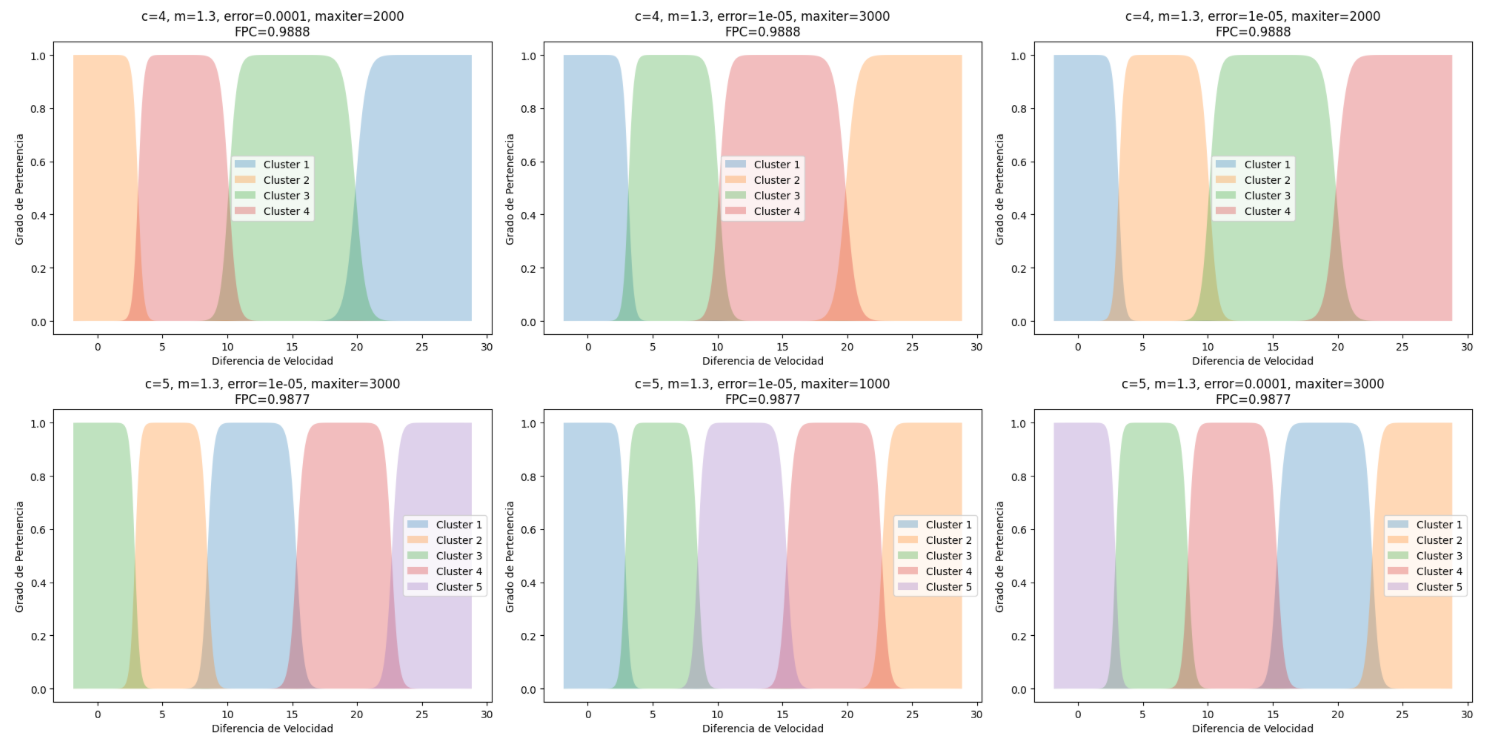
\includegraphics[width=1\linewidth]{./figs/herramientas/desarrollo/grid_search.png}
	\caption[Ejemplo de parámetros de \ac{fcm} probados]{Ejemplo de parámetros de \ac{fcm} probados}
    \label{fig:grid_search}
\end{figure}
\vspace{2em}

Una vez implementado y aplicado el algoritmo de \ac{fcm} a las diferentes métricas de telemetría, se añadió la información del agrupamiento resultante a la estructura de datos en Rust denominada 'Analysis'. Este nuevo añadido permitió almacenar para cada punto de las distancias comunes cuales son los distintos valores de pertenencia a cada una de las agrupaciones. En la \autoref{fig:modelo_de_datos_clustering} se muestra un diagrama de esta estructura, ilustrando cómo se integra la información del agrupamiento con la estructura de datos ya existente.

\begin{figure}[H]
	\centering
	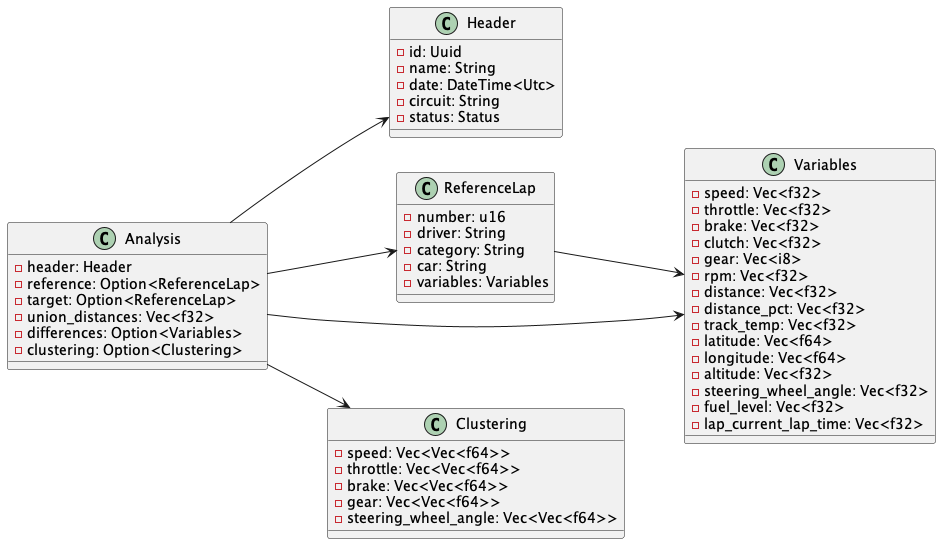
\includegraphics[width=1\linewidth]{./figs/herramientas/desarrollo/modelo_de_datos_clustering.png}
	\caption[Modelo de Datos con Agrupamiento Difuso]{Modelo de Datos con Agrupamiento Difuso}
    \label{fig:modelo_de_datos_clustering}
\end{figure}





\newpage

\section{Hito 4: Construcción de Sugerencias en Lenguaje Natural}

En este hito, se desarrolló un enfoque sistemático para asignar etiquetas en lenguaje natural a cada punto de diferencias de las variables de telemetría. Este enfoque está orientado a guiar al piloto en los ajustes necesarios para mejorar sus tiempos. A continuación se presenta la tabla resumen del hito.

\begin{table}[H]
\centering
\begin{tabular}{|l|c|}
\hline
\textbf{Título} & Construcción de Sugerencias en Lenguaje Natural \\ \hline
\textbf{Código} & \textit{SO4} \\ \hline
\textbf{Historias de Usuario} & 2 \\ \hline
\textbf{Sprints} & 27-28 \\ \hline
\end{tabular}
\caption{Resumen de la sección: Construcción de Sugerencias en Lenguaje Natural}
\label{tab:resumen_so4}
\end{table}

A continuación se detallan las historias de usuario que conformaron este hito.

\subsection{Asignación de etiquetas semántica a las agrupaciones de diferencias}
\begin{table}[H]
\centering
\begin{tabular}{|l|p{10cm}|}
\hline
\multicolumn{2}{|c|}{\textbf{Historia de Usuario 11}} \\ \hline
\textbf{Nombre:} & Asignación de etiquetas semánticas a las agrupaciones de diferencias \\ \hline
\textbf{Descripción:} & Como cliente del proyecto, quiero que se asignen etiquetas semánticas a las agrupaciones de diferencias de las variables de telemetría, para proporcionar una interpretación clara y útil de los resultados del análisis. \\ \hline
\textbf{Prioridad:} & P1 \\ \hline
\textbf{Talla:} & S \\ \hline
\textbf{Sprints:} & 27 \\ \hline
\end{tabular}
\caption{Historia de Usuario 11}
\label{tab:asignacion_semanitca_agrupaciones}
\end{table}

Para llevar a cabo esta historia de usuario, se partió de las diferencias de variables agrupadas mediante el algoritmo \ac{fcm}. Con el objetivo de asignar etiquetas automáticamente a las agrupaciones, independientemente de lo que signifique semánticamente la variable, se decidió utilizar tres etiquetas base: ``mantener'', ``aumentar'' y ``disminuir''.

Dado que cada vector de diferencias puede tener un número distinto de agrupaciones, optimizado en base a la prueba de parámetros, fue necesario desarrollar una estrategia para realizar esta asignación. Primero, se ordenaron los grupos de manera ascendente según el valor de sus centroides. Luego, se identificó el grupo que contenía el valor de diferencia 0 con el mayor grado de pertenencia. Este grupo fue etiquetado como ``mantener'', ya que representaba los datos más cercanos a la no diferencia.

Para los grupos con centroides menores que el de ``mantener'', se asignó la etiqueta ``disminuir''. Esto se debe a que una diferencia negativa indica que la variable está por encima del valor de referencia, por lo tanto, es necesario tomar medidas para reducir su valor. Por otro lado, los grupos con centroides mayores que el de ``mantener'' fueron etiquetados como ``aumentar'', ya que una diferencia positiva sugiere que el valor actual es inferior al de referencia y, por tanto, se requiere incrementarlo.

Adicionalmente, para los grupos más alejados de ``mantener'', se utilizó una nomenclatura incrementada para indicar la intensidad del cambio necesario. Así, los grupos a la izquierda de ``disminuir'' se etiquetaron como ``disminuir+'', ``disminuir++'', ``disminuir+++'', etc, y de manera análoga, los grupos a la derecha de ``aumentar'' se etiquetaron como ``aumentar+'', ``aumentar++'', ``aumentar+++'', etc. Esta metodología sistemática permitió crear el \autoref{alg:asignacion_etiquetas} para la asignación automática de etiquetas.

\begin{algorithm}[H]
\SetKwInOut{Input}{Entrada}
\SetKwInOut{Output}{Salida}
\caption{Asignación de Etiquetas Semánticas a los Clusters}
\label{alg:asignacion_etiquetas}

\Input{Centroides de los clusters $cntr$}
\Output{Etiquetas semánticas para cada cluster}

Ordenar los clusters por el valor de sus centroides\;
$sorted\_indices \leftarrow$ Índices de $cntr$ ordenados ascendentemente\;
$sorted\_cntr \leftarrow cntr[sorted\_indices]$\;

Inicializar $mantener\_index \leftarrow None$\;

\For{$i \leftarrow 0$ \KwTo longitud($sorted\_cntr$) - 1}{
    \If{$sorted\_cntr[i] \leq 0$}{
        $mantener\_index \leftarrow i$\;
    }
}

Inicializar lista vacía $etiquetas$\;

\For{$i \leftarrow 0$ \KwTo longitud($sorted\_cntr$) - 1}{
    \If{$mantener\_index = None$}{
        $etiqueta \leftarrow$ ``aumentar'' + ``+'' * $i$\;
    }
    \ElseIf{$mantener\_index = $ longitud($sorted\_cntr$) - 1}{
        $etiqueta \leftarrow$ ``disminuir'' + ``+'' * $(longitud($sorted\_cntr$) - 1 - i)$\;
    }
    \Else{
        \If{$i = mantener\_index$}{
            $etiqueta \leftarrow$ ``mantener''\;
        }
        \ElseIf{$i < mantener\_index$}{
            $etiqueta \leftarrow$ ``disminuir'' + ``+'' * $(mantener\_index - i - 1)$\;
        }
        \Else{
            $etiqueta \leftarrow$ ``aumentar'' + ``+'' * $(i - mantener\_index - 1)$\;
        }
    }
    Añadir $etiqueta$ a $etiquetas$\;
}

\Return $etiquetas$\;
\end{algorithm}




\subsection{Utilización de conjuntos difusos para pertenencia múltiple}
\begin{table}[H]
\centering
\begin{tabular}{|l|p{10cm}|}
\hline
\multicolumn{2}{|c|}{\textbf{Historia de Usuario 12}} \\ \hline
\textbf{Nombre:} & Utilización de conjuntos difusos para pertenencia múltiple \\ \hline
\textbf{Descripción:} & Como cliente del proyecto, quiero que se utilicen conjuntos difusos para permitir la pertenencia múltiple de puntos de diferencia a varias categorías, con el fin de proporcionar sugerencias más precisas y detalladas. \\ \hline
\textbf{Prioridad:} & P2 \\ \hline
\textbf{Talla:} & S \\ \hline
\textbf{Sprints:} & 28 \\ \hline
\end{tabular}
\caption{Historia de Usuario 12}
\label{tab:utilizacion_conjuntos_difusos}
\end{table}

En esta historia de usuario, se aprovechó la lógica difusa para mejorar la precisión y detalle de las sugerencias proporcionadas al piloto. Los conjuntos difusos permiten que un punto pertenezca a múltiples categorías de manera parcial, lo cual es fundamental para representar situaciones donde una variable de telemetría se encuentra en una zona intermedia entre dos categorías. Para implementar esto, se definió un umbral de pertenencia a partir del cual se considera significativa la pertenencia a otra clase. 

Se justificó que un umbral de 0,25 sería adecuado porque permite identificar con suficiente claridad las tendencias significativas sin incluir demasiadas pertenencias parciales que podrían complicar la interpretación. Este umbral permite diferenciar adecuadamente entre una pertenencia principal y pertenencias parciales significativas.

El proceso de asignación de etiquetas lingüísticas consistió en combinar la clase principal con las clases parciales significativas para cada punto de diferencia. Esto se realizó ordenando los grados de pertenencia de mayor a menor y asignando la etiqueta de la clase con el mayor grado de pertenencia como etiqueta principal. Luego, se evaluaron los siguientes grados de pertenencia para determinar si eran significativos según el umbral definido, y se añadieron las tendencias correspondientes a la etiqueta principal. El \autoref{alg:asignacion_etiquetas_difusas} ilustra cómo se llevó a cabo dicho proceso.

\begin{algorithm}[H]
\SetKwInOut{Input}{Entrada}
\SetKwInOut{Output}{Salida}
\caption{Asignación de Etiquetas Lingüísticas con Conjuntos Difusos}
\label{alg:asignacion_etiquetas_difusas}

\Input{Lista de diferencias $diferencias$, Matriz de pertenencias $pertenencias$, Lista de etiquetas $etiquetas$, Umbral $umbral$}
\Output{Lista de etiquetas finales $etiquetas\_finales$}

Inicializar lista vacía $etiquetas\_finales$\;

\ForEach{$diferencia \, d$ en $diferencias$}{
    Ordenar las pertenencias de $d$ de mayor a menor\;
    $clase\_principal \leftarrow$ clase con mayor pertenencia a $d$\;
    $grado\_principal \leftarrow$ pertenencia de $d$ en la $clase\_principal$\;
    $etiqueta \leftarrow etiquetas[clase\_principal]$\;
    
    Inicializar cadena vacía $tendencia$\;
    
    \ParaCada{$clase\_secundaria$ en las clases restantes}{
        $grado\_secundario \leftarrow$ pertenencia de $d$ en la $clase\_secundaria$\;
        \Si{$grado\_secundario > umbral$ \textbf{y} $tendencia$ está vacía}{
            $tendencia \leftarrow etiquetas[clase\_secundaria]$\;
            \Si{$tendencia$ comienza con la misma raíz que $etiqueta$}{
                $etiqueta \leftarrow etiqueta + `` con tendencia a '' + tendencia$\;
            }
        }
    }
    
    Añadir $etiqueta$ a $etiquetas\_finales$\;
}

\Return $etiquetas\_finales$\;
\end{algorithm}

Las etiquetas generadas mediante este algoritmo aportan información detallada y precisa, que luego puede ser traducida a lenguaje natural de forma sencilla, proporcionando sugerencias claras y comprensibles para el piloto. Por ejemplo, etiquetas como ``mantener con tendencia a aumentar'' o ``aumentar con tendencia a aumentar+'' permiten comunicar de manera efectiva las acciones necesarias para mejorar el rendimiento.


En la \autoref{fig:etiquetas_difusas} se presenta un ejemplo detallado de la aplicación de los algoritmos \autoref{alg:asignacion_etiquetas} y \autoref{alg:asignacion_etiquetas_difusas} sobre las diferencias de la variable velocidad tras aplicar \ac{fcm}. Se identificaron cinco agrupaciones, donde la tercera, que contiene los valores cercanos a cero, fue etiquetada como ``mantener''. Las agrupaciones a la izquierda fueron etiquetadas como ``disminuir'' y ``disminuir+'', ya que abarcan el espectro de diferencias negativas. Las agrupaciones a la derecha fueron etiquetadas como ``aumentar'' y ``aumentar+'', cubriendo el espectro de diferencias positivas. El eje Y representa el grado de pertenencia a cada agrupación, y el eje X muestra las diferencias de velocidad. Los centroides de las agrupaciones se indican con estrellas verdes. Los puntos rojos representan diferencias que superan el umbral de pertenencia múltiple, indicando una tendencia significativa hacia otra clase, mientras que los puntos negros indican pertenencia exclusiva a una única clase.


\begin{figure}[H]
	\centering
	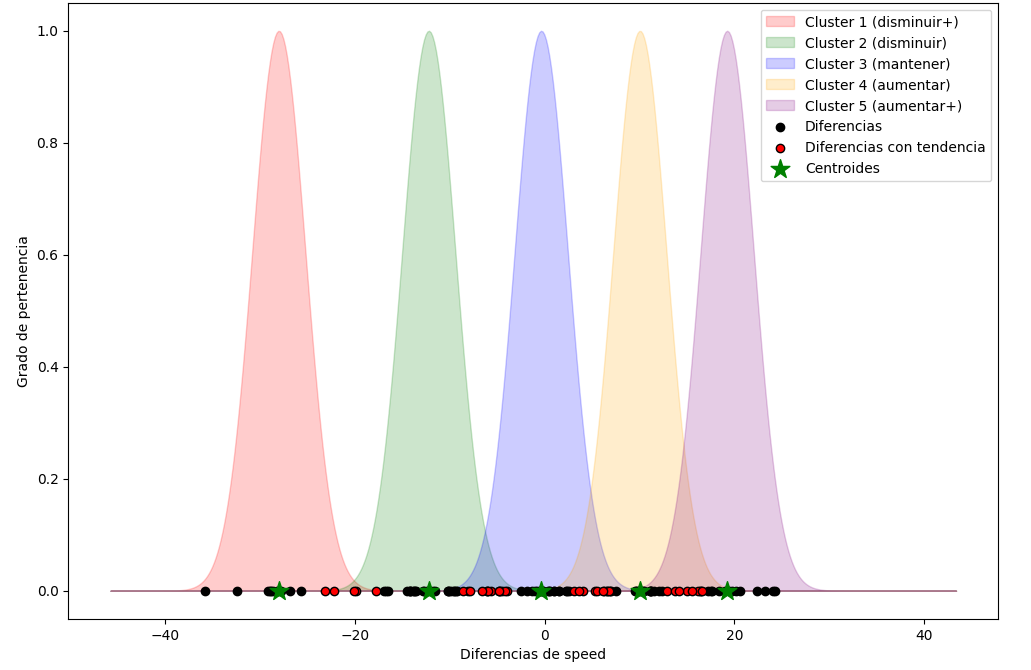
\includegraphics[width=1\linewidth]{./figs/herramientas/desarrollo/etiquetas_difusas.png}
	\caption[Diagrama de dispersión con conjuntos difusos para la variable ``speed'']{Diagrama de dispersión con conjuntos difusos para la variable ``speed''}
    \label{fig:etiquetas_difusas}
\end{figure}


Finalmente, se añadió la información del etiquetado al modelo de clases en Rust, utilizando enums con métodos de creación e incremento, como se muestra en la \autoref{fig:diagrama_clases_etiquetas}.

\begin{figure}[H]
	\centering
	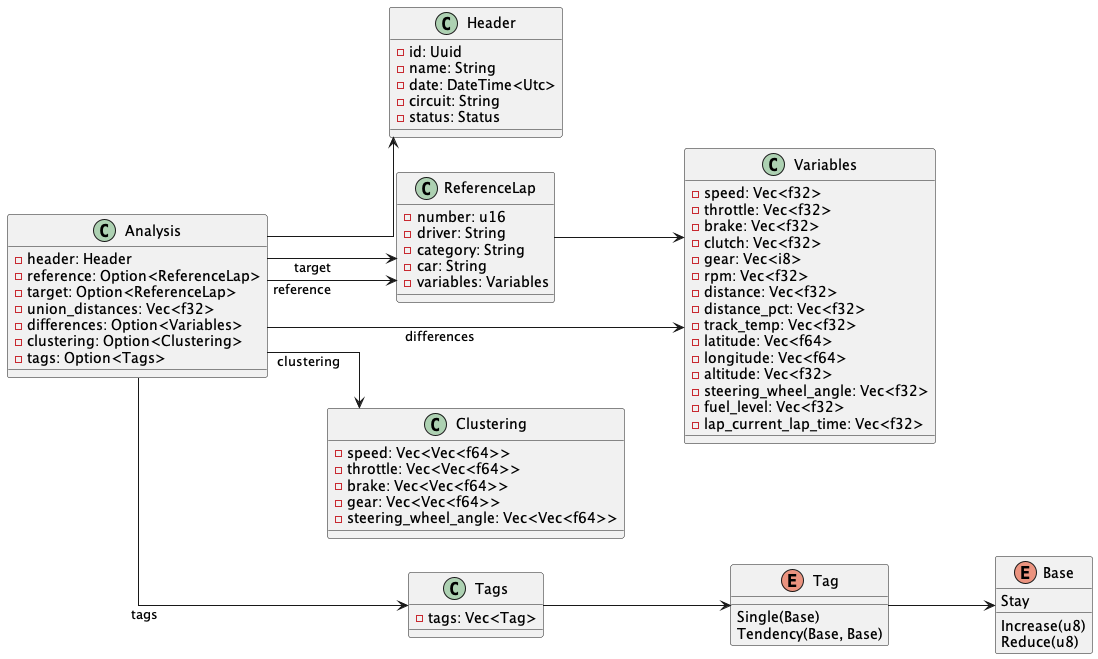
\includegraphics[width=1\linewidth]{./figs/herramientas/desarrollo/diagrama_clases_etiquetas.png}
	\caption[Diagrama de clases con etiquetas asignadas]{Diagrama de clases con etiquetas asignadas}
    \label{fig:diagrama_clases_etiquetas}
\end{figure}


\newpage

\section{Hito 5: Desarrollo de aplicación web \textit{(SO5)}}

El desarrollo de la aplicación web se centró en la creación de una plataforma accesible y funcional para gestionar y analizar los datos de telemetría extraídos. Este hito incluyó la implementación de varias características clave que permitieron a los usuarios subir y gestionar ficheros de telemetría, realizar análisis comparativos entre diferentes vueltas y visualizar los resultados de manera intuitiva. A continuación se presenta la tabla resumen de este hito:

\begin{table}[H]
\centering
\begin{tabular}{|l|c|}
\hline
\textbf{Título} & Desarrollo de Aplicación Web \\ \hline
\textbf{Código} & \textit{SO5} \\ \hline
\textbf{Historias de Usuario} & 4 \\ \hline
\textbf{Sprints} & 29-34 \\ \hline
\end{tabular}
\caption{Resumen de la sección: Desarrollo de Aplicación Web}
\label{tab:desarrollo_aplicacion_web}
\end{table}

% Párrafo introductorio a las historias de usuario
A continuación se detallan las historias de usuario que conformaron este hito, enfocadas en la creación y mejora de la aplicación web para gestionar y analizar los datos de telemetría de manera eficiente.

% Historia de Usuario 1
\subsection{Diseño de la arquitectura de la aplicación web}
\begin{table}[H]
\centering
\begin{tabular}{|l|p{10cm}|}
\hline
\multicolumn{2}{|c|}{\textbf{Historia de Usuario 12}} \\ \hline
\textbf{Nombre:} & Diseño de la arquitectura de la aplicación web \\ \hline
\textbf{Descripción:} & Como cliente del proyecto, quiero un diseño robusto de la arquitectura de la aplicación web, que garantice escalabilidad, seguridad y facilidad de mantenimiento, para asegurar un desempeño óptimo y una experiencia de usuario eficiente. \\ \hline
\textbf{Prioridad:} & P1 \\ \hline
\textbf{Talla:} & L \\ \hline
\textbf{Sprints:} & 29 \\ \hline
\end{tabular}
\caption{Historia de Usuario 12}
\label{tab:diseno_arquitectura_web}
\end{table}

En esta historia de usuario se diseñó la arquitectura de la aplicación web, asegurando escalabilidad, seguridad y facilidad de mantenimiento, para ofrecer un desempeño óptimo y una experiencia de usuario eficiente. A continuación, se presenta una descripción detallada de cómo se estructuró y construyó la arquitectura, tanto para el \textit{backend} como para el \textit{frontend}.

\subsubsection*{Backend}
\begin{itemize}
    \item \textbf{Estructura}: se organizó siguiendo los principios de \ac{ddd}, permitiendo una clara separación de responsabilidades y facilitando la reutilización de componentes. La organización principal es la siguiente:
    \begin{itemize}
        \item \textbf{api}: Maneja la infraestructura de la aplicación, ensamblando componentes, controladores y suscriptores.
        \item \textbf{ibt\_extractor}: Gestiona la extracción y conversión de datos de telemetría.
        \item \textbf{main.rs}: Punto de entrada principal de la aplicación \textit{backend}.
        \item \textbf{backend-config.yaml}: Archivo de configuración que incluye parámetros específicos para la ejecución del \textit{backend}.
    \end{itemize}
    \item \textbf{Axum y Green Threads}: se eligió \textit{Axum} \cite{axum_github} debido a su rendimiento y capacidad de manejo multihilo, desarrollado por los creadores de \textit{Tokio} \cite{tokio}, librería de referencia para programación concurrente en Rust (\autoref{fig:rust}). \textit{Axum} se destacó por su robustez y eficiencia en la gestión de solicitudes concurrentes, esencial para asegurar un desempeño óptimo en el procesamiento de datos de telemetría. Se utilizaron \textit{green threads} \cite{green_thread} de Rust para crear un servidor multihilo, permitiendo gestionar múltiples hilos de ejecución de manera eficiente. Los \textit{green threads} son una abstracción de hilos de bajo nivel que permiten un manejo más eficiente de las tareas concurrentes.
        \begin{figure}[H]
        	\centering
        	
\includegraphics[width=0.3\linewidth]{./figs/herramientas/desarrollo/rust.png}
        	\caption[Logotipo de Rust]{Logotipo de Rust}
            \label{fig:rust}
        \end{figure}
    \item \textbf{Controladores y Suscriptores de Eventos}: La capa de infraestructura del \textit{backend} se diseñó para implementar los servicios expuestos por la capa de aplicación de dos formas:
    \begin{itemize}
        \item \textbf{Controladores}: Implementan las \ac{api} \ac{rest} clásicas, permitiendo la comunicación entre el cliente y el servidor a través de \ac{http}. Estos controladores gestionan solicitudes, procesan datos y devuelven respuestas adecuadas.
        \item \textbf{Suscriptores}: Servicios que se ejecutan de manera reactiva ante eventos del sistema. Estos suscriptores escuchan eventos específicos y desencadenan acciones en respuesta, permitiendo una arquitectura más flexible y reactiva.
    \end{itemize}
    \item \textbf{Arquitectura Hexagonal}: Los elementos de la arquitectura hexagonal \cite{hexagonal_architecture} se definieron mediante repositorios y otros puertos como interfaces de dominio. La arquitectura hexagonal, también conocida como Arquitectura de Puertos y Adaptadores, promueve la separación de la lógica de negocio del resto del sistema, facilitando el mantenimiento y la escalabilidad. Esta arquitectura se complementa perfectamente con los principios de \ac{ddd}, que enfoca el diseño del software en el dominio central de la aplicación y su lógica de negocio.

    En esta arquitectura, los puertos actúan como interfaces que definen las operaciones disponibles para el dominio. Los adaptadores implementan estos puertos y permiten que la lógica de negocio interactúe con servicios externos, bases de datos y otros sistemas. Este enfoque asegura que los componentes del dominio no estén acoplados a la infraestructura técnica, como bases de datos o servicios externos.
    
    En esta implementación:
    \begin{itemize}
        \item \textbf{Repositorios}: Definidos como interfaces en el dominio, permiten acceder a los datos de una manera desacoplada. Las implementaciones específicas de estos repositorios se encuentran en la capa de infraestructura, garantizando que el dominio no dependa de detalles específicos de almacenamiento.
        \item \textbf{Servicios externos}: Se accede a través de interfaces definidas en el dominio. Estas interfaces son implementadas por adaptadores en la capa de infraestructura, permitiendo cambiar fácilmente los servicios externos sin afectar la lógica de negocio.
    \end{itemize}
    
    Este diseño permitió una clara separación de responsabilidades, facilitando pruebas unitarias, mantenimiento y escalabilidad de la aplicación.
\end{itemize}

\subsubsection*{Frontend}
\begin{itemize}
        \item \textbf{Estructura}: se eligió el framework \textit{Yew} \cite{yew}, que utiliza una arquitectura similar a \textit{React} \cite{react} y \textit{Elm} \cite{elm_components}. \textit{Yew} permite estructurar la aplicación con componentes reutilizables, facilitando el desarrollo y mantenimiento de la interfaz de usuario. La organización principal es la siguiente:
    \begin{itemize}
        \item \textbf{src}: Contiene el código fuente del \textit{frontend}, dividido en:
        \begin{itemize}
            \item \textbf{infrastructure}: Maneja componentes, repositorios y configuración del \textit{frontend}.
            \item \textbf{main.rs}: Punto de entrada principal de la aplicación \textit{frontend}.
        \end{itemize}
        \item \textbf{assets}: Archivos estáticos como \ac{css}, imágenes y scripts.
        \item \textbf{frontend-config.yaml}: Archivo de configuración que incluye parámetros específicos para la ejecución del \textit{frontend}.
    \end{itemize}
    \item \textbf{Componentes Reutilizables en Yew}:\textit{Yew} (\autoref{fig:yew}) permite la creación de componentes reutilizables, lo que facilita el desarrollo y mantenimiento de la interfaz de usuario. Los componentes en \textit{Yew} son unidades independientes de funcionalidad que se pueden combinar para construir interfaces complejas de manera modular. Esto proporciona varios beneficios:
    \begin{itemize}
        \item \textbf{Reutilización}: Los componentes se pueden reutilizar en diferentes partes de la aplicación, reduciendo la duplicación de código y facilitando el mantenimiento.
        \item \textbf{Modularidad}: La aplicación se puede dividir en componentes más pequeños y manejables, lo que mejora la organización del código y facilita la comprensión y el desarrollo.
        \item \textbf{Facilidad de Mantenimiento}: Los cambios en la lógica de un componente no afectan a otros componentes, lo que reduce el riesgo de errores y facilita la actualización de la aplicación.
        \begin{figure}[H]
        	\centering
        	
\includegraphics[width=0.3\linewidth]{./figs/herramientas/desarrollo/yew.png}
        	\caption[Logotipo de Yew]{Logotipo de Yew}
            \label{fig:yew}
        \end{figure}
    \end{itemize}
    \item \textbf{Integración con el Backend}: El \textit{frontend} implementa los repositorios contra la \ac{api} \ac{rest} del \textit{backend}, mientras que el \textit{backend} lo hace contra MongoDB \cite{mongodb}. Ambos serializan y deserializan los objetos de la misma manera, aprovechando todos los elementos desarrollados en los hitos anteriores desde ambos lados. Esto asegura que cualquier cambio en la lógica de negocio se refleje tanto en el cliente como en el servidor de manera uniforme.
    \item \textbf{WebAssembly}: Se utilizó \ac{wasm} (\autoref{fig:wasm}) para permitir la ejecución de código Rust tanto en el \textit{backend} como en el \textit{frontend}, facilitando la reutilización de la lógica de negocio y mejorando la eficiencia del desarrollo. \ac{wasm} es un estándar que permite ejecutar código de bajo nivel en los navegadores web, proporcionando un rendimiento cercano al nativo. Esto permite que lenguajes como Rust, conocidos por su seguridad y eficiencia, se utilicen en el desarrollo de aplicaciones web complejas. Al utilizar \ac{wasm}, se garantiza que la lógica de negocio implementada en Rust se pueda ejecutar de manera eficiente en el navegador, proporcionando una experiencia de usuario fluida y reduciendo la carga de trabajo del \textit{backend}.
        \begin{figure}[H]
        \centering
        
\includegraphics[width=0.3\linewidth]{./figs/herramientas/desarrollo/wasm.png}
        \caption[Logotipo de \ac{wasm}]{Logotipo de \ac{wasm}}
        \label{fig:wasm}
        \end{figure}
\end{itemize}

\subsubsection*{Beneficios de la Arquitectura Diseñada}
La arquitectura diseñada garantizó:
\begin{itemize}
    \item \textbf{Escalabilidad}: La estructura modular y el uso de tecnologías eficientes permitieron el crecimiento y adaptación de la aplicación según las necesidades.
    \item \textbf{Seguridad}: La configuración adecuada y el uso de tecnologías robustas aseguraron la protección de los datos y las operaciones del sistema.
    \item \textbf{Facilidad de Mantenimiento}: La separación clara de responsabilidades y la reutilización de componentes facilitaron la gestión y actualización de la aplicación.
    \item \textbf{Desempeño Óptimo}: La selección cuidadosa de tecnologías y la implementación eficiente aseguraron un rendimiento excelente de la aplicación.
    \item \textbf{Experiencia de Usuario Eficiente}: La interfaz intuitiva y la rapidez de respuesta proporcionaron una experiencia de usuario satisfactoria y efectiva.
\end{itemize}

% Historia de Usuario 2
\subsection{Gestión de Ficheros de Telemetría}
\begin{table}[H]
\centering
\begin{tabular}{|l|p{10cm}|}
\hline
\multicolumn{2}{|c|}{\textbf{Historia de Usuario 13}} \\ \hline
\textbf{Nombre:} & Gestión de Ficheros de Telemetría \\ \hline
\textbf{Descripción:} & Como usuario, quiero poder subir ficheros de telemetría, visualizar las vueltas contenidas en ellos, y tener la capacidad de borrar ficheros completos o vueltas individuales, para gestionar mis datos de manera eficiente. \\ \hline
\textbf{Prioridad:} & P1 \\ \hline
\textbf{Talla:} & M \\ \hline
\textbf{Sprints:} & 30 \\ \hline
\end{tabular}
\caption{Historia de Usuario 13}
\label{tab:gestion_ficheros_telemetria}
\end{table}

\subsubsection*{Backend}

Para la implementación de la funcionalidad de gestión de ficheros de telemetría en el \textit{backend}, se diseñaron e implementaron los servicios necesarios dentro de la capa de aplicación. Se creó el módulo \texttt{ibt\_extractor}, que se encarga de recibir un objeto que implementa los traits \texttt{Read} y \texttt{Seek} y devuelve una estructura \texttt{IBTFile} con los datos extraídos. Dado que este servicio utiliza intensivamente la entrada y salida, se implementó como un suscriptor de eventos. Concretamente, este servicio escucha el evento \texttt{FileUploaded}, que se emite cuando se han transferido todos los bytes del fichero \texttt{ibt} desde el equipo del cliente. La extracción se ejecuta en un hilo separado, devolviendo un código \texttt{CONTINUE} de HTTP para evitar el bloqueo del cliente.

Se creó una estructura \texttt{File} para representar un fichero de telemetría dentro del dominio, independiente del sistema \textit{iRacing}. Esta estructura contiene atributos como el \texttt{SHA256} del fichero, su nombre, su estado y la fecha de creación. Cuando un usuario sube un fichero, se crea automáticamente un objeto \texttt{File} en el sistema cuyo \texttt{id} corresponde al \texttt{SHA256} del fichero \texttt{ibt} (para evitar redundancia de información) y se inicializa con el estado \texttt{Accepted}. Al completarse la extracción, se emite un evento \texttt{IbtExtracted}, al que está suscrito el servicio \texttt{validate} del módulo \texttt{file}. Este servicio cambia el estado del fichero de \texttt{Accepted} a \texttt{Success}. En caso de error durante la extracción, otro servicio de la capa de aplicación del dominio \texttt{File}, denominado \texttt{mark\_as\_error}, escucha el evento y marca el fichero como erróneo, junto con un mensaje explicativo de la razón. En la \autoref{fig:seq_file_upload} se muestra el diagrama de secuencia de lo anterior.

\begin{figure}[H]
\centering
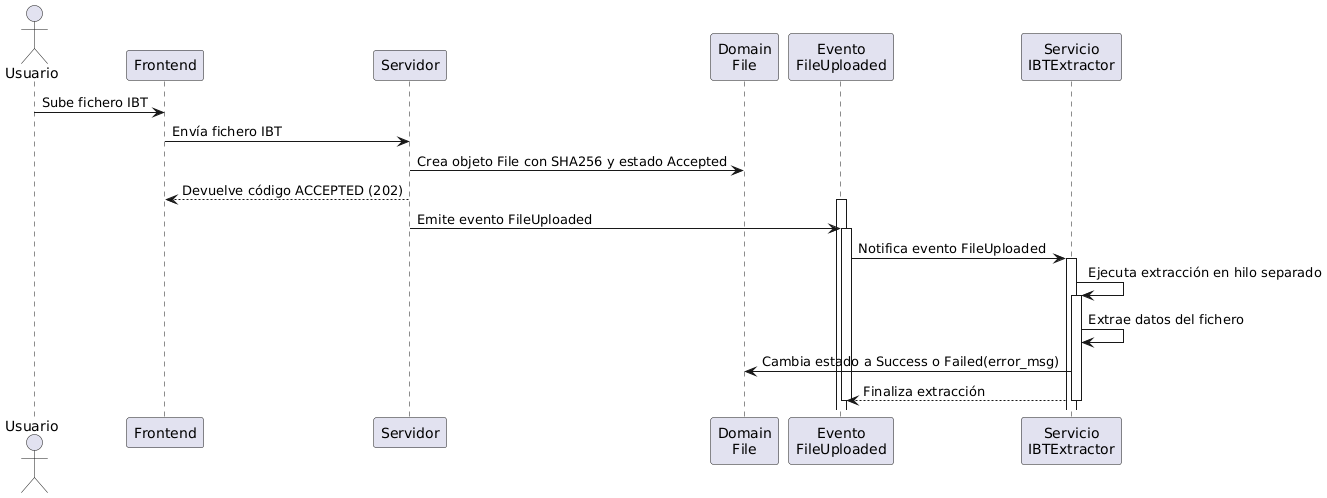
\includegraphics[width=1\linewidth]{./figs/herramientas/desarrollo/seq_file_upload.png}
\caption[Diagrama de secuencia de subida de un fichero]{Diagrama de secuencia de subida de un fichero}
\label{fig:seq_file_upload}
\end{figure}

Cuando un fichero se marca como \texttt{Success}, se emite otro evento que se encarga de almacenar todas las vueltas (\texttt{Laps}) contenidas en el fichero extraído en el sistema. Además, si un \texttt{File} se elimina, se emite un evento \texttt{FileDeleted}, al cual está suscrito un servicio del módulo \texttt{Lap}, que elimina del sistema todas las vueltas (\texttt{Laps}) cuyo \texttt{file\_id} corresponde al fichero eliminado. Se puede ver este funcionamiento en la \autoref{fig:seq_file_store_and_delete_laps}.

\begin{figure}[H]
\centering
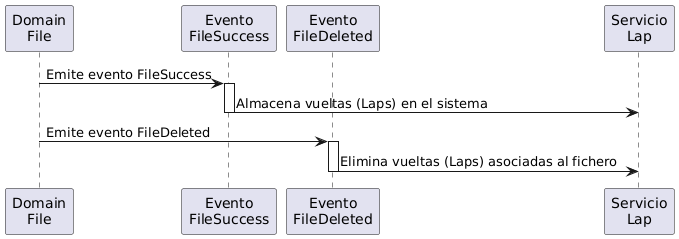
\includegraphics[width=1\linewidth]{./figs/herramientas/desarrollo/seq_file_store_and_delete_laps.png}
\caption[Diagrama de secuencia de guardado y borrado de vueltas]{Diagrama de secuencia de guardado y borrado de vueltas}
\label{fig:seq_file_store_and_delete_laps}
\end{figure}

El módulo \texttt{lap} se encarga de gestionar las vueltas (\texttt{Laps}) extraídas de los ficheros de telemetría. Este módulo incluye servicios para crear, eliminar y encontrar vueltas, así como para obtener los encabezados de las vueltas. En el dominio, se definen las estructuras de las vueltas, incluyendo los encabezados y las variables asociadas a cada vuelta. Los repositorios se utilizan para abstraer el acceso a los datos y facilitar la persistencia y recuperación de las vueltas en el sistema.

\subsubsection*{Frontend}
El componente de subida de ficheros permite al usuario seleccionar un archivo desde su dispositivo y enviar una petición al \textit{backend} para subirlo. Dado que el comportamiento predeterminado de un componente \texttt{form} en \ac{html} es redirigir a la página especificada en el atributo \texttt{action} una vez que la petición se completa, se tuvo que manejar manualmente la subida multipart para mantener la interfaz de usuario sin interrupciones. Esto se logró implementando funciones asíncronas que procesan la subida de archivos y gestionan las respuestas del servidor sin bloquear la interfaz.


En la pantalla de \textit{Files} (\autoref{fig:front_file}), además del componente de subida, se incluye una lista de los ficheros de telemetría almacenados en el sistema. Cada entrada de la lista muestra el nombre del fichero y ofrece dos opciones: 
\begin{itemize}
    \item \textbf{Borrar Fichero}: Permite al usuario eliminar un fichero del sistema. Al seleccionar esta opción, se emite el evento \texttt{FileDeleted}, desencadenando la eliminación de todas las vueltas (\texttt{Laps}) asociadas a dicho fichero.
    \item \textbf{Visualizar Vueltas}: Proporciona al usuario la capacidad de ver todas las vueltas contenidas en el fichero seleccionado. Esto se realiza mediante un botón que redirige a una pantalla donde se detallan todas las vueltas asociadas al fichero.
\end{itemize}

\begin{figure}[H]
\centering
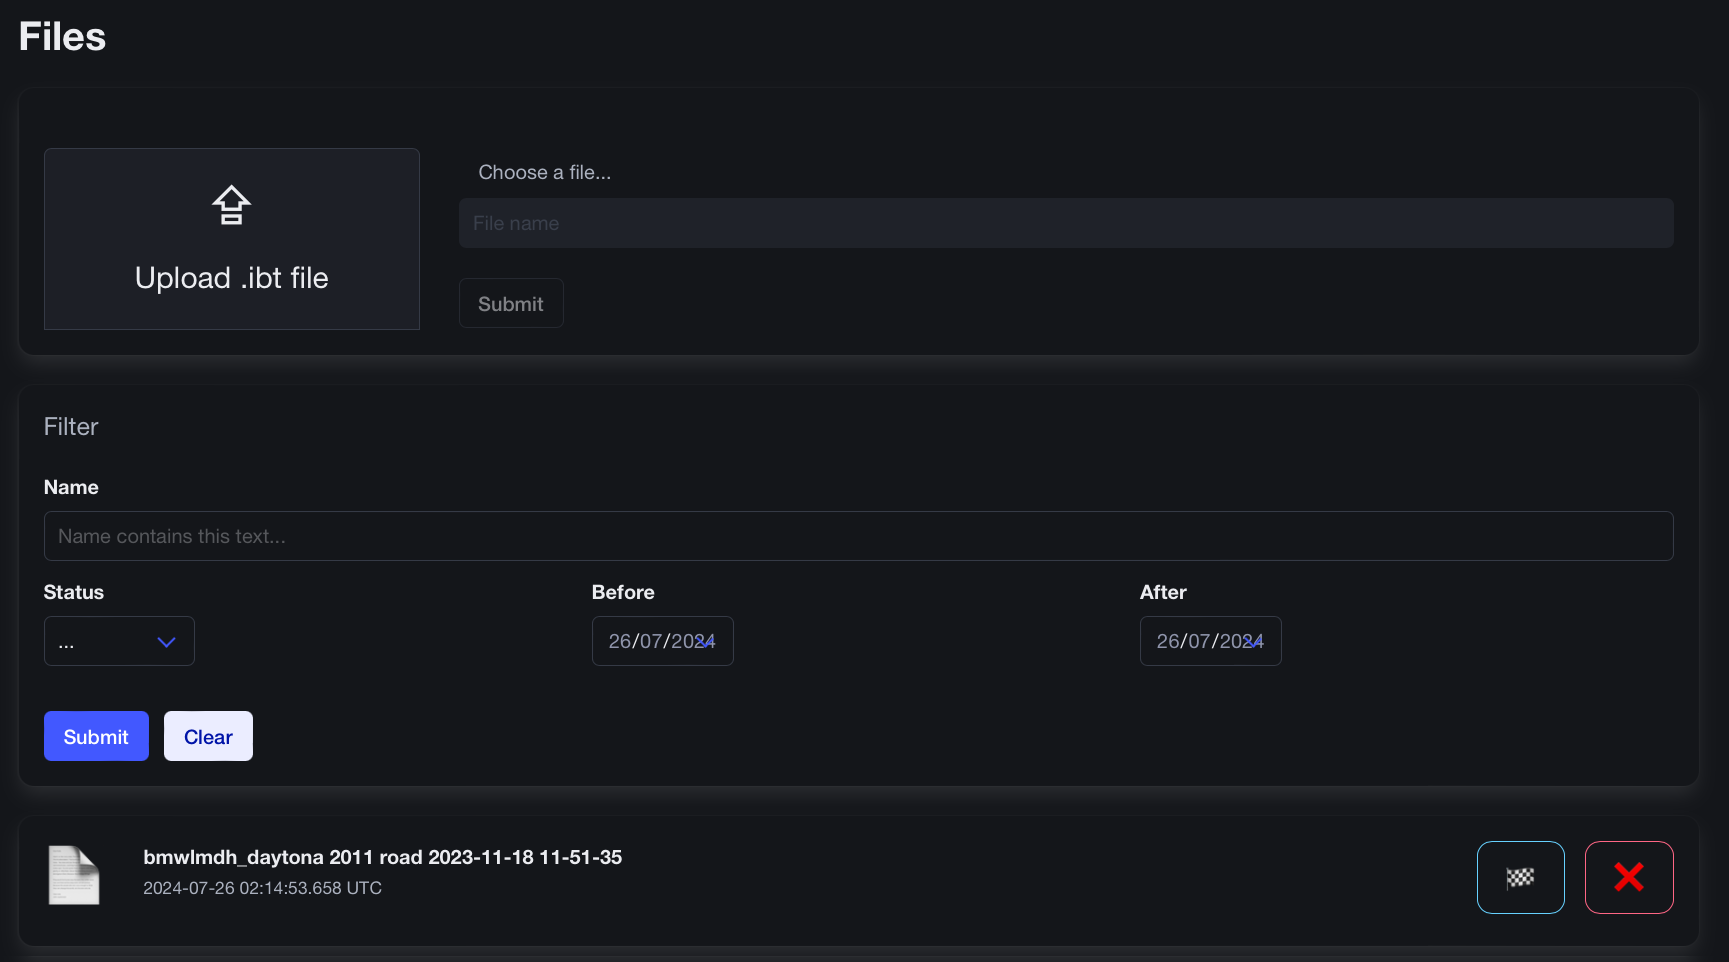
\includegraphics[width=1\linewidth]{./figs/herramientas/desarrollo/front_file.png}
\caption[Pantalla de Files]{Pantalla de Files}
\label{fig:front_file}
\end{figure}

En la \autoref{fig:front_file_accepted} se muestra el icono de fichero aceptado, que indica que el archivo de telemetría ha sido correctamente recibido por el sistema y está pendiente de procesamiento.

\begin{figure}[H]
\centering

\includegraphics[width=1\linewidth]{./figs/herramientas/desarrollo/front_file_accepted.png}
\caption[Fichero en estado Accepted]{Fichero en estado Accepted}
\label{fig:front_file_accepted}
\end{figure}

En la \autoref{fig:front_file_success} se presenta el icono de fichero satisfactorio, señalando que el archivo ha sido procesado con éxito y sus datos han sido extraídos y almacenados correctamente.

\begin{figure}[H]
\centering

\includegraphics[width=1\linewidth]{./figs/herramientas/desarrollo/front_file_success.png}
\caption[Fichero en estado Success]{Fichero en estado Success}
\label{fig:front_file_success}
\end{figure}

% Historia de Usuario 3
\subsection{Realización de análisis comparativo entre vueltas}
\begin{table}[H]
\centering
\begin{tabular}{|l|p{10cm}|}
\hline
\multicolumn{2}{|c|}{\textbf{Historia de Usuario 14}} \\ \hline
\textbf{Nombre:} & Realización de análisis comparativo entre vueltas \\ \hline
\textbf{Descripción:} & Como usuario, quiero poder realizar análisis comparativos entre dos vueltas seleccionadas, pudiendo filtrar por diferentes atributos. \\ \hline
\textbf{Prioridad:} & P1 \\ \hline
\textbf{Talla:} & S \\ \hline
\textbf{Sprints:} & 30-31 \\ \hline
\end{tabular}
\caption{Historia de Usuario 14}
\label{tab:analisis_comparativo_vueltas}
\end{table}

\subsubsection*{Backend}

El módulo \texttt{Analysis} encapsuló todos los servicios necesarios para realizar un análisis comparativo entre dos vueltas. El proceso de creación de un análisis comienza con la recepción de un identificador (ID), un nombre, una fecha, un ID de la vuelta de referencia y un ID de la vuelta a comparar.

El módulo de análisis llama al servicio de búsqueda de vueltas del módulo \texttt{Lap} para comprobar la existencia de ambas vueltas. Además, verifica que ambas vueltas pertenezcan al mismo circuito para garantizar la validez de la comparación. Una vez confirmadas estas condiciones, se crea una instancia de la estructura \texttt{Analysis} y se emite el evento \texttt{AnalysisCreated}. El \texttt{Analysis} comienza con estado Accepted

En este punto, se devuelve un código \ac{http} 202 (Accepted) al cliente, con el fin de evitar tiempos de bloqueo en la interfaz de usuario. El servicio \texttt{analyze} del módulo \texttt{Analysis}, implementado como un suscriptor, escucha este evento y realiza el análisis en segundo plano. En la \autoref{fig:seq_create_analysis} se muestra el diagrama de secuencia que representa lo anterior.

\begin{figure}[H]
\centering
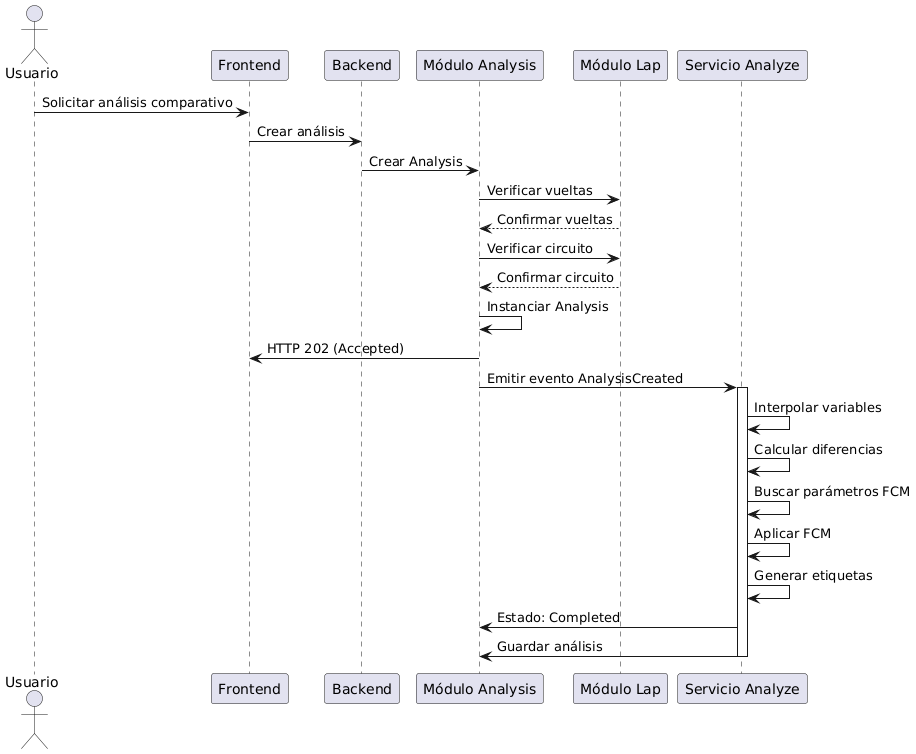
\includegraphics[width=0.6\linewidth]{./figs/herramientas/desarrollo/seq_create_analysis.png}
\caption[Diagrama de secuencia de creación de un Análisis]{Diagrama de secuencia de creación de un Análisis}
\label{fig:seq_create_analysis}
\end{figure}

El análisis comienza interpolando los valores de las variables de la vuelta de referencia y la vuelta a comparar en función de la unión de las distancias. Posteriormente, calcula el vector de diferencias, ejecuta la búsqueda de parámetros del algoritmo \ac{fcm}, aplica \ac{fcm} con los parámetros óptimos y genera las etiquetas correspondientes. Finalmente, la instancia de \texttt{Analysis} pasa del estado \texttt{Accepted} a \texttt{Completed}.

Una vez completado el análisis, toda la información generada se guardó en el sistema, y el análisis quedó disponible para su consulta posterior.

\subsubsection*{Frontend}

Para el desarrollo del frontend, se implementó una pantalla dedicada a la gestión de análisis comparativos entre vueltas de telemetría. Esta pantalla muestra las vueltas disponibles en el sistema y permite al usuario seleccionar dos de ellas para realizar un análisis. La funcionalidad principal de esta pantalla se centró en la selección de vueltas y la solicitud de creación de análisis comparativos.

Primero, se diseñó e implementó una lista de vueltas disponibles en el sistema. Esta lista proporciona información detallada de cada vuelta, permitiendo al usuario identificar rápidamente las vueltas que desea comparar. Para facilitar la búsqueda de vueltas específicas, se implementó una funcionalidad de filtrado. Este filtrado permite al usuario buscar vueltas que cumplan determinados criterios, tales como el nombre del circuito, el nombre del piloto, o el tiempo de la vuelta (\autoref{fig:front_analysis_list}).

\begin{figure}[H]
\centering
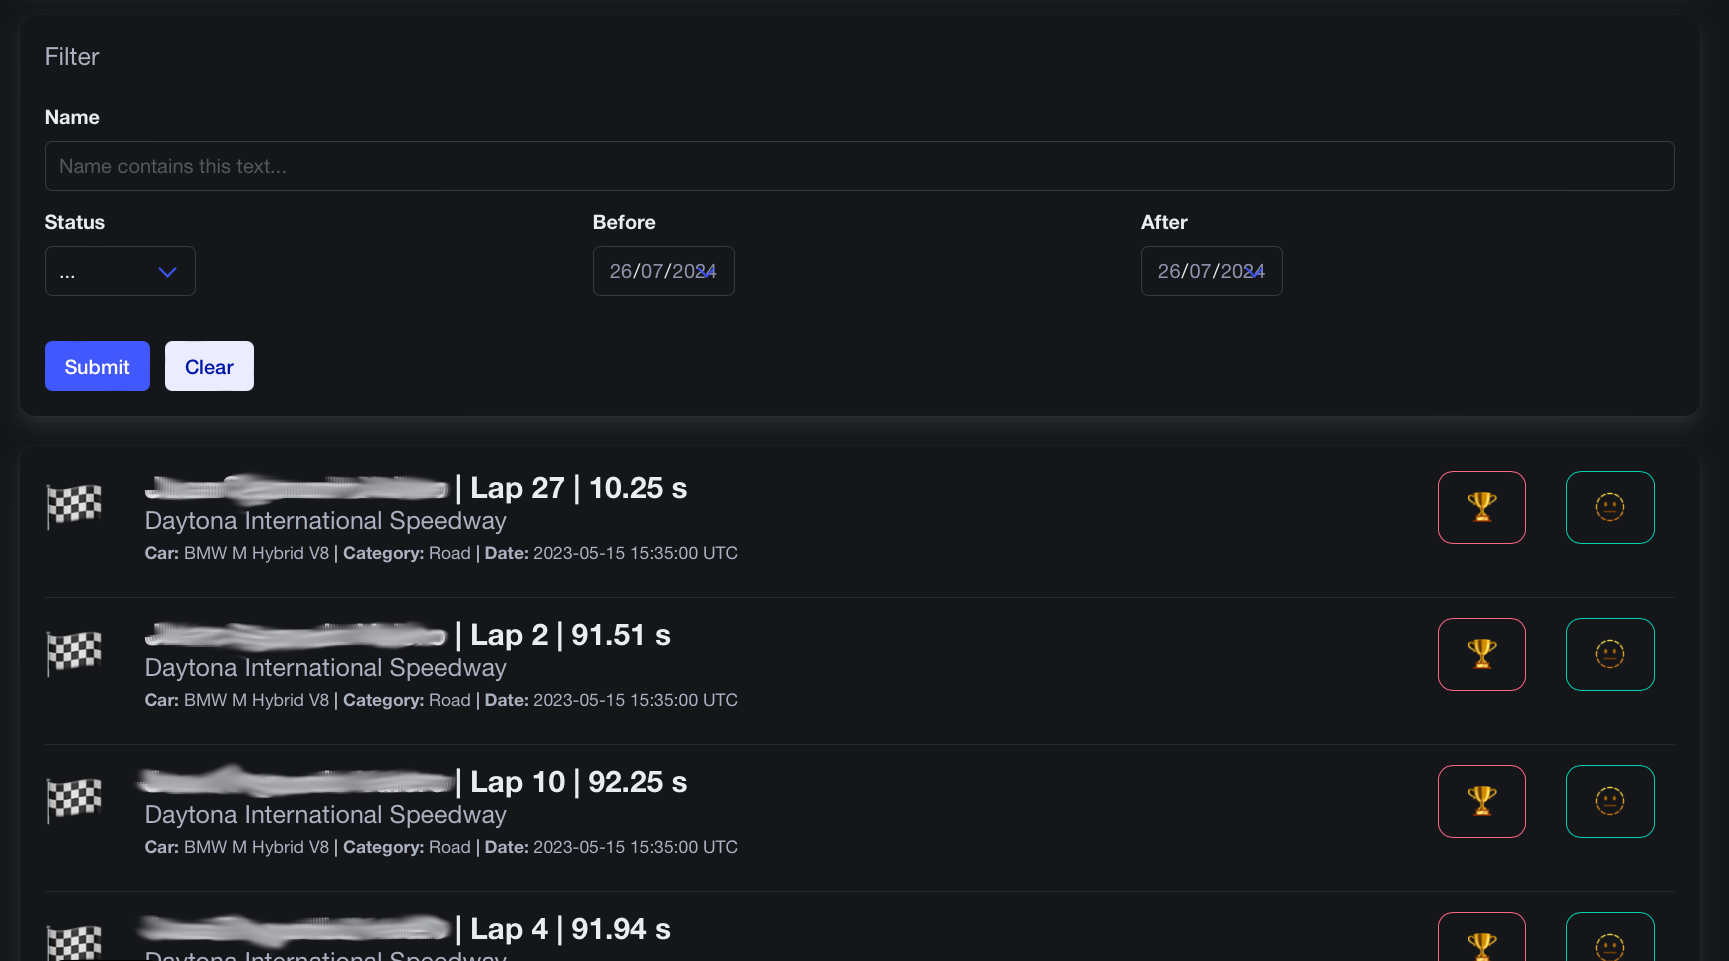
\includegraphics[width=0.6\linewidth]{./figs/herramientas/desarrollo/front_analysis_list.png}
\caption[Listado de vueltas en un Análisis]{Listado de vueltas en un Análisis}
\label{fig:front_analysis_list}
\end{figure}

Cada elemento de la lista de vueltas incluye dos botones al final: uno para seleccionar la vuelta como vuelta de referencia y otro para seleccionarla como vuelta a comparar (\autoref{fig:front_analysis_btn}). Al pulsar el botón de vuelta de referencia, la vuelta seleccionada se añade como la vuelta de referencia para el análisis. De manera similar, al pulsar el botón de vuelta a comparar, la vuelta seleccionada se añade como la vuelta a comparar para el análisis. Esta implementación permite al usuario seleccionar fácilmente las vueltas que desea comparar sin necesidad de cambiar de pantalla o realizar acciones adicionales complicadas.

\begin{figure}[H]
\centering

\includegraphics[width=0.3\linewidth]{./figs/herramientas/desarrollo/front_analysis_btn.png}
\caption[Botones de las vueltas en un Análisis]{Botones de las vueltas en un Análisis}
\label{fig:front_analysis_btn}
\end{figure}

Una vez que el usuario ha seleccionado las vueltas de referencia y a comparar, puede proceder a completar la creación del análisis en el componente de selección de vueltas (\autoref{fig:front_analysis_creator}). El componente de selección de vueltas permite al usuario ingresar un nombre y una fecha para el análisis, asegurando que los detalles del análisis sean claros y fácilmente identificables.

\begin{figure}[H]
\centering
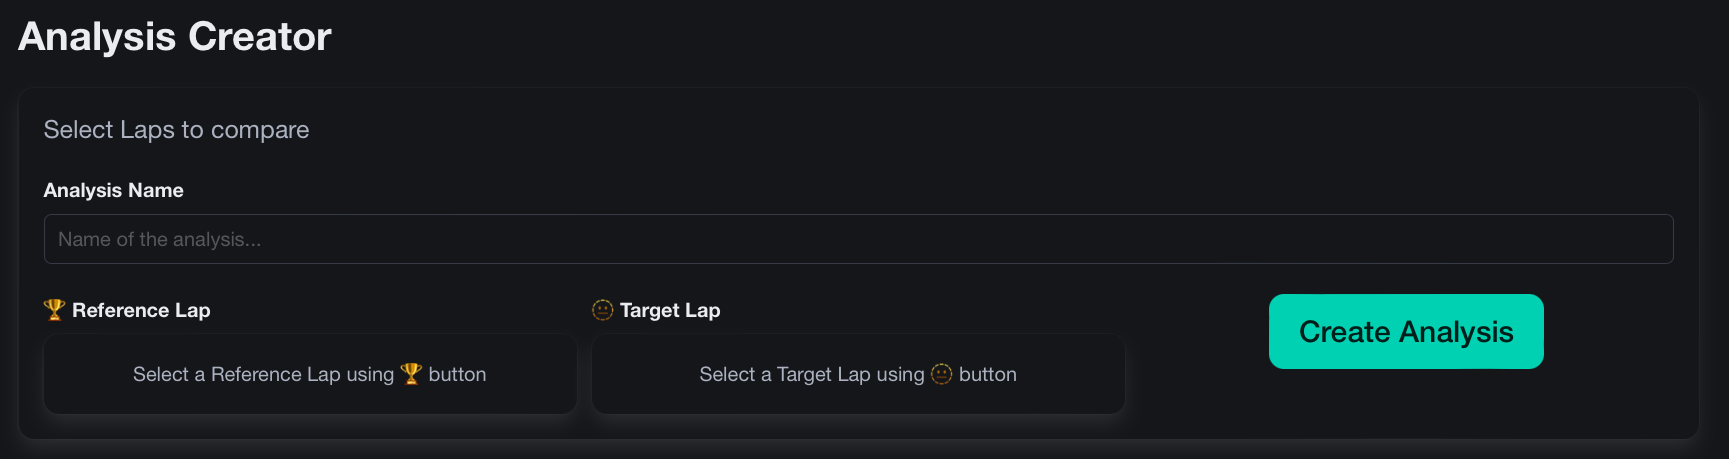
\includegraphics[width=0.6\linewidth]{./figs/herramientas/desarrollo/front_analysis_creator.png}
\caption[Selector de vueltas en un Análisis]{Selector de vueltas en un Análisis}
\label{fig:front_analysis_creator}
\end{figure}

Finalmente, al pulsar el botón de enviar, el frontend envía una solicitud al backend para crear el análisis comparativo entre las dos vueltas seleccionadas. Esta solicitud se gestiona de manera asíncrona, asegurando que la interfaz de usuario permanezca receptiva y evitando tiempos de espera prolongados para el usuario.

La pantalla de gestión de análisis comparativos se diseñó para proporcionar una experiencia de usuario intuitiva y eficiente, permitiendo a los usuarios realizar análisis detallados de su rendimiento de manera rápida y sencilla.

% Historia de Usuario 4
\subsection{Visualización de resultados del análisis en un cuadro de mandos}
\begin{table}[H]
\centering
\begin{tabular}{|l|p{10cm}|}
\hline
\multicolumn{2}{|c|}{\textbf{Historia de Usuario 15}} \\ \hline
\textbf{Nombre:} & Visualización de resultados del análisis en un cuadro de mandos \\ \hline
\textbf{Descripción:} & Como usuario, quiero poder visualizar los resultados del análisis de telemetría en un cuadro de mandos interactivo para facilitar la interpretación y toma de decisiones basadas en los datos. \\ \hline
\textbf{Prioridad:} & P1 \\ \hline
\textbf{Talla:} & M \\ \hline
\textbf{Sprints:} & 32-34 \\ \hline
\end{tabular}
\caption{Historia de Usuario 15}
\label{tab:visualizacion_resultados_dashboard}
\end{table}

Para la implementación de la funcionalidad de visualización de resultados del análisis de telemetría en un cuadro de mandos interactivo, se desarrolló un componente \textit{Yew} compuesto por varios sub-componentes. Esta historia de usuario se centró exclusivamente en el \textit{frontend}, dado que ya existían todos los componentes necesarios en el \textit{backend}.

El cuadro de mandos se diseñó para mostrar los diagramas de dispersión de las variables más representativas según el consultor del proyecto. Estas variables son velocidad, porcentaje del pedal de aceleración pisado, porcentaje del pedal de freno pisado, marcha y ángulo de giro del volante. Estas son las mismas variables que utilizan la mayoría de los sistemas comerciales.

Para cada una de estas cinco variables, se mostró un diagrama de dispersión. En estos diagramas, el eje x representa la distancia o el punto del circuito donde se encuentra el vehículo, medido en metros. Los ejes y se dividieron en dos: uno que muestra los valores de la variable para ambas vueltas y otro que presenta el valor de la diferencia en una escala diferente. Se apilaron los diagramas de dispersión de manera que se puedan observar de forma conjunta, tal y como se muestra en la \autoref{fig:dashboard}. Además, se sincronizó el cursor de todas las gráficas para que se moviera simultáneamente, aprovechando que el eje x es la distancia para todas las variables. Esta sincronización facilita la comparación en tiempo real de las variables a lo largo del circuito.

Otro componente esencial del cuadro de mandos es un \textit{canvas \ac{html}} con el circuito dibujado. En este \textit{canvas \ac{html}}, se añadió un puntero que, al moverse, también mueve el cursor de los diagramas de dispersión al punto correspondiente. Para lograr esta interacción, se utilizaron enlaces entre JavaScript y Rust mediante \ac{wasm}.

Debajo del circuito, se implementaron unos botones de radio que permiten seleccionar una de las variables analizadas. Al seleccionar una variable, el circuito pinta cada uno de sus puntos de un color específico en función de la agrupación a la que pertenece y el grado de pertenencia. Esta visualización facilita la identificación de los puntos donde hay mayores diferencias en la variable seleccionada, proporcionando una vista clara y detallada del rendimiento en el circuito.

Por último, debajo del selector de variables, se añadió un panel que muestra, en lenguaje natural, una acción recomendada en función de la etiqueta lingüística asignada. Esta funcionalidad ofrece una guía clara y directa sobre las acciones a tomar para mejorar el rendimiento basado en el análisis de telemetría. El cudro de mandos completo se muestra en la \autoref{fig:dashboard}.
\begin{figure}[H]
\centering
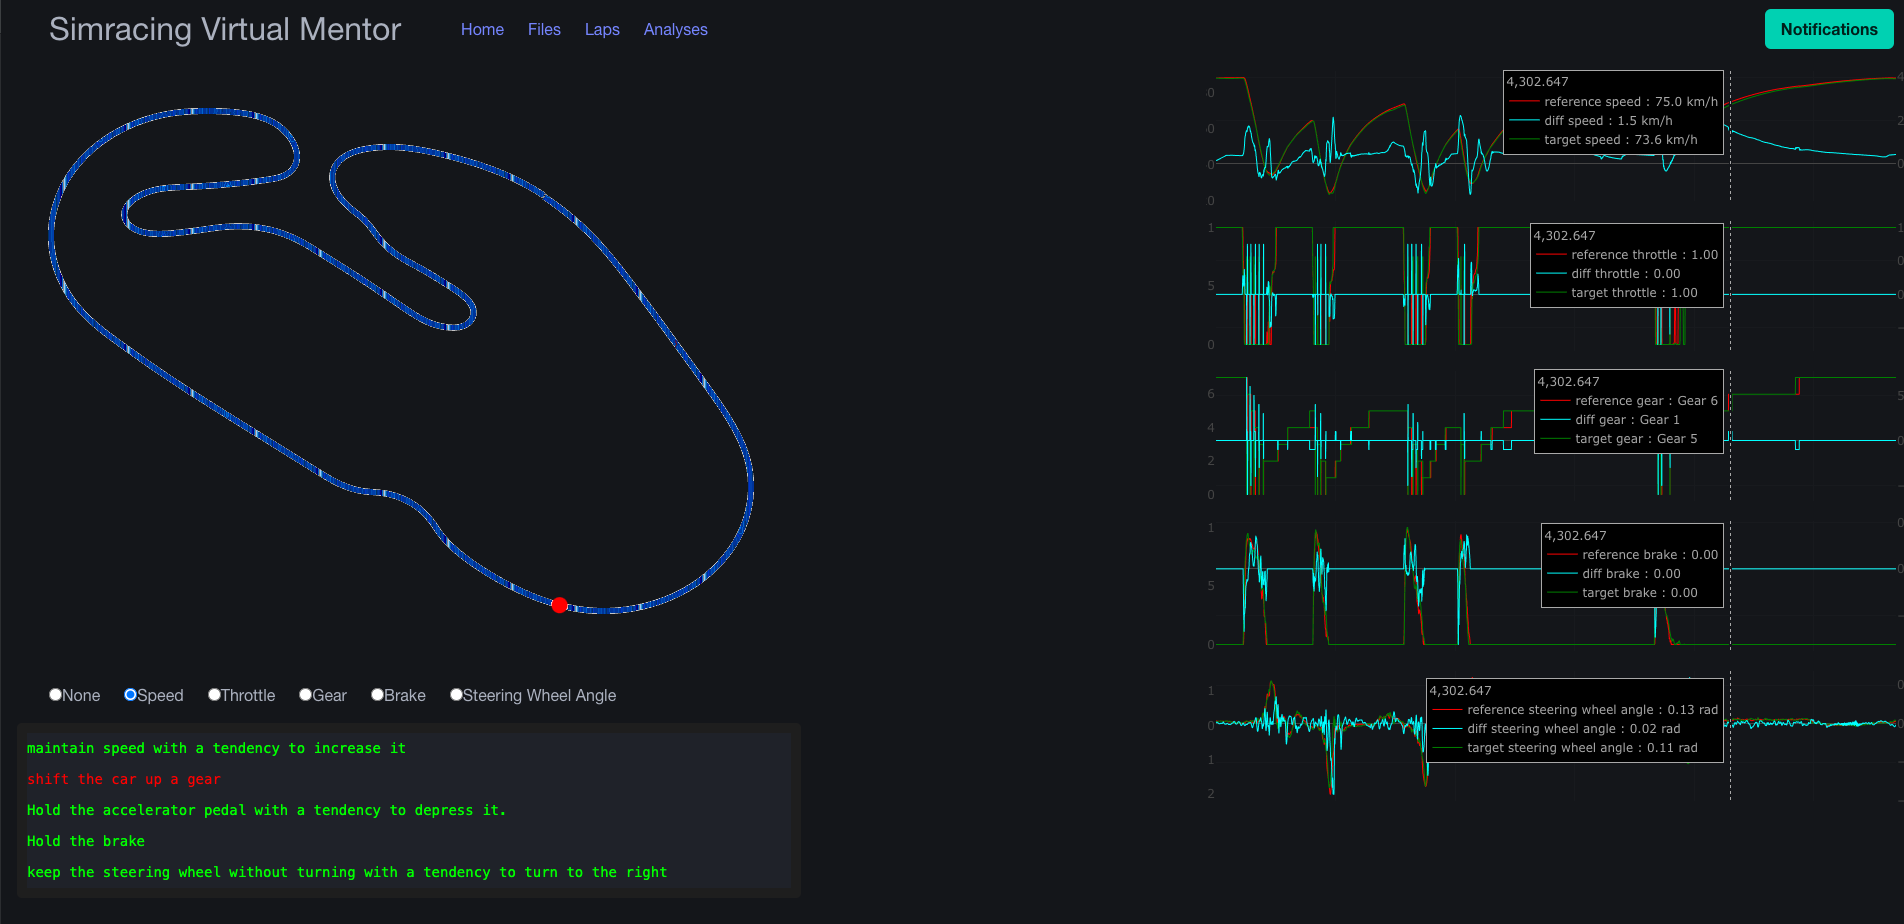
\includegraphics[width=1\linewidth]{./figs/herramientas/desarrollo/svm.png}
\caption[Cuadro de Mandos]{Cuadro de Mandos}
\label{fig:dashboard}
\end{figure}

La integración de estos componentes en un cuadro de mandos interactivo ha permitido una visualización detallada y comprensible de los datos de telemetría, facilitando la interpretación y la toma de decisiones basadas en los datos analizados.